\begin{chapterpage}{Distributions of random variables}
  \chaptertitle[30]{Distributions of random \titlebreak{} variables}
  \label{ch_distributions}
  \chaptersection{normalDist}
\chaptersection{distributionofxbar}
  \chaptersection{geomDist}
  \chaptersection{binomialModel}
  \chaptersection{distributionphat}
\end{chapterpage}
\renewcommand{\chapterfolder}{ch_distributions}
\index{distribution!normal|(}

\chapterintro{fill in}


%__________________________________________________
\section[Normal distribution]{Normal distribution }
\label{normalDist}

\sectionintro{
Questions


\subsection*{Learning objectives}
\begin{enumerate}
\item Calculate and interpret a Z-score.

\item Understand that Z-scores are unitless (standard units) and are not affected by change of units.

\item Use the normal model to approximate a distribution where appropriate.

\item Find probabilities and percentiles using the normal approximation.

\item Find the value that corresponds to a given percentile when the distribution is approximately normal.  

\end{enumerate}
}



\Comment{placement of figure}

%%
\subsection{Normal distribution model}

Among all the distributions we see in practice, one is overwhelmingly the most common. The symmetric, unimodal, bell curve is ubiquitous throughout statistics. Indeed it is so common, that people often know it as the \term{normal curve} or \termsub{normal distribution}{distribution!normal},\footnote{It is also introduced as the Gaussian distribution after Frederic Gauss, the first person to formalize its mathematical expression.} shown in Figure~\ref{simpleNormal}. 

\begin{figure}
\centering
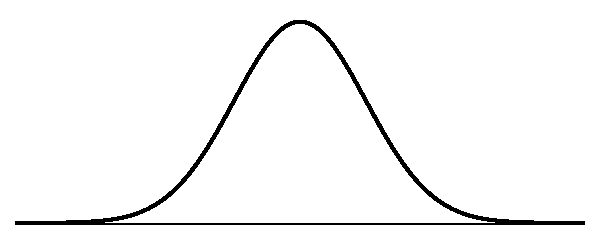
\includegraphics[width=0.6\textwidth]{ch_distributions/figures/simpleNormal/simpleNormal}
\caption{A normal curve.}
\label{simpleNormal}
\end{figure}

The normal distribution model always describes a symmetric, unimodal, bell-shaped curve. However, these curves can look different depending on the details of the model. Specifically, the normal distribution model can be adjusted using two parameters: mean and standard deviation. As you can probably guess, changing the mean shifts the bell curve to the left or right, while changing the standard deviation stretches or constricts the curve. Figure~\ref{twoSampleNormals} shows the normal distribution with mean $0$ and standard deviation $1$ in the left panel and the normal distributions with mean $19$ and standard deviation $4$ in the right panel. Figure~\ref{twoSampleNormalsStacked} shows these distributions on the same axis.
\newpage

\begin{figure}[hht]
\centering
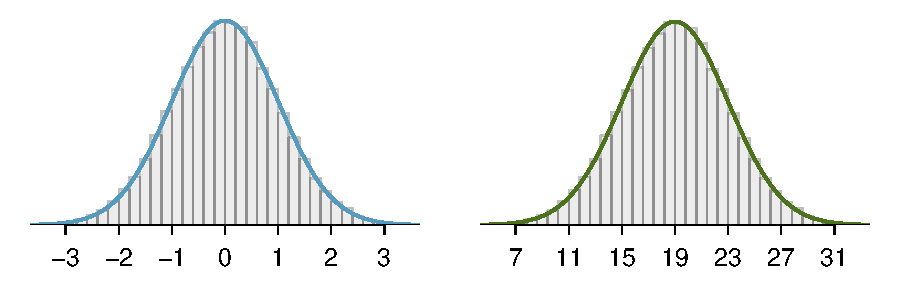
\includegraphics[width=0.95\textwidth]{ch_distributions/figures/twoSampleNormals/twoSampleNormals}
\caption{Both curves represent the normal distribution, however, they differ in their center and spread. The normal distribution with mean 0 and standard deviation 1 is called the \term{standard normal distribution}.}
\label{twoSampleNormals}
\end{figure}

\begin{figure}[hht]
\centering
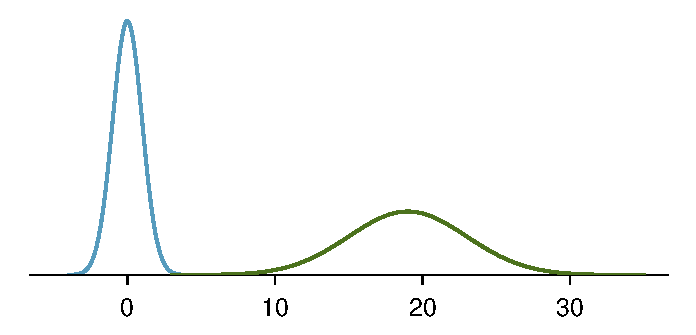
\includegraphics[width=0.67\textwidth]{ch_distributions/figures/twoSampleNormalsStacked/twoSampleNormalsStacked}
\caption{The normal models shown in Figure~\ref{twoSampleNormals} but plotted together and on the same scale.}
\label{twoSampleNormalsStacked}
\end{figure}

Because the mean and standard deviation describe a normal distribution exactly, they are called the distribution's \termsub{parameters}{parameter}.


\begin{onebox}{Normal distribution facts}
Many variables are nearly normal, but none are exactly normal. The normal distribution, while never perfect, provides very close approximations for a variety of scenarios. We will use it in data exploration and to solve important problems in statistics.\vspace{0.7mm}\end{onebox}
\textA{\newpage}

%%
%%
\subsection{Standardizing with Z-scores}

\begin{examplewrap}
\begin{nexample}{Table~\vref{satACTstats} shows the mean and standard deviation for total scores on the SAT and ACT. The distribution of SAT and ACT scores are both nearly normal. Suppose Ann scored 1800 on her SAT and Tom scored 24 on his ACT. Who performed better?}\label{actSAT}
Since the two distributions are on different scales, we use the standard deviation as a guide. Ann is 1 standard deviation above average on the SAT: $1500 + 300=1800$. Tom is 0.6 standard deviations above the mean on the ACT: $21+0.6\times 5=24$. In Figure~\ref{satActNormals}, we can see that Ann tends to do better with respect to everyone else than Tom did, so her score was better.
\end{nexample}
\end{examplewrap}

\begin{table}
\centering
\begin{tabular}{l r r}
  \hline
  & SAT & ACT \\
  \hline
Mean \hspace{0.3cm} & 1500 & 21 \\
SD & 300 & 5 \\
   \hline
\end{tabular}
\caption{Mean and standard deviation for the SAT and ACT.}
\label{satACTstats}
\end{table}

\begin{figure}
\centering
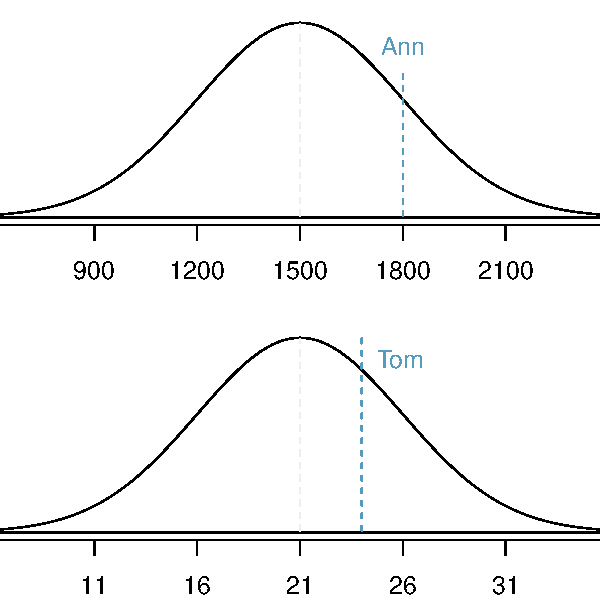
\includegraphics[width=65mm]{ch_distributions/figures/satActNormals/satActNormals}
\caption{Ann's and Tom's scores shown with the distributions of SAT and ACT scores.}
\label{satActNormals}
\end{figure}

Example~\ref{actSAT} used a standardization technique called a Z-score, a method most commonly employed for nearly normal observations but that may be used with any distribution. The \term{Z-score}\index{Z@$Z$} of an observation is defined as the number of standard deviations it falls above or below the mean. If the observation is one standard deviation above the mean, its Z-score is 1. If it is 1.5 standard deviations \emph{below} the mean, then its Z-score is -1.5. If $x$ is an observation from a distribution with mean $\mu$ and standard deviation $\sigma$, we define the Z-score mathematically as
\begin{eqnarray*}
Z = \frac{x-\mu}{\sigma}
\end{eqnarray*}
Using $\mu_{SAT}=1500$, $\sigma_{SAT}=300$, and $x_{Ann}=1800$, we find Ann's Z-score:
\begin{eqnarray*}
Z_{Ann} = \frac{x_{Ann} - \mu_{SAT}}{\sigma_{SAT}} = \frac{1800-1500}{300} = 1
\end{eqnarray*}

\begin{onebox}{The Z-score}
The Z-score of an observation is the number of standard deviations it falls above or below the mean. We compute the Z-score for an observation $x$ that follows a distribution with mean $\mu$ and standard deviation $\sigma$ using
\begin{eqnarray*}
Z = \frac{x-\mu}{\sigma}
\end{eqnarray*}\end{onebox}

\begin{exercisewrap}
\begin{nexercise}
Use Tom's ACT score, 24, along with the ACT mean of 21 and standard deviation of 5 to compute his Z-score.\footnotemark
\end{nexercise}
\end{exercisewrap}
\footnotetext{$Z_{Tom} = \frac{x_{Tom} - \mu_{ACT}}{\sigma_{ACT}} = \frac{24 - 21}{5} = 0.6$}

Observations above the mean always have positive Z-scores while those below the mean have negative Z-scores. If an observation is equal to the mean (e.g. SAT score of 1500), then the Z-score is $0$.

\begin{exercisewrap}
\begin{nexercise}
Let $X$ represent a random variable from a distribution with $\mu = 3$ and $\sigma = 2$, and suppose we observe $x=5.19$. (a) Find the Z-score of $x$. (b) Use the Z-score to determine how many standard deviations above or below the mean $x$~falls.\footnotemark
\end{nexercise}
\end{exercisewrap}
\footnotetext{(a) Its Z-score is given by $Z = \frac{x-\mu}{\sigma} = \frac{5.19 - 3}{2} = 2.19/2 = 1.095$. (b) The observation $x$ is 1.095 standard deviations \emph{above} the mean. We know it must be above the mean since $Z$ is positive.}

\begin{exercisewrap}
\begin{nexercise} \label{headLZScore}
Head lengths of brushtail possums follow a nearly normal distribution with mean 92.6 mm and standard deviation 3.6 mm. Compute the Z-scores for possums with head lengths of 95.4 mm and 85.8 mm.\footnotemark
\end{nexercise}
\end{exercisewrap}
\footnotetext{For $x_1=95.4$ mm: $Z_1 = \frac{x_1 - \mu}{\sigma} = \frac{95.4 - 92.6}{3.6} = 0.78$. For $x_2=85.8$ mm: $Z_2 = \frac{85.8 - 92.6}{3.6} = -1.89$.}

We can use Z-scores to roughly identify which observations are more unusual than others. One observation $x_1$ is said to be more unusual than another observation $x_2$ if the absolute value of its Z-score is larger than the absolute value of the other observation's Z-score: $|Z_1| > |Z_2|$. This technique is especially insightful when a distribution is symmetric.

\begin{exercisewrap}
\begin{nexercise}
Which of the observations in Guided Practice~\ref{headLZScore} is more unusual?\footnotemark
\end{nexercise}
\end{exercisewrap}
\footnotetext{Because the \emph{absolute value} of Z-score for the second observation is larger than that of the first, the second observation has a more unusual head length.}

%%
%%
\subsection{Normal probability table}

\begin{examplewrap}
\begin{nexample}{Ann from Example~\ref{actSAT} earned a score of 1800 on her SAT with a corresponding $Z=1$. She would like to know what percentile she falls in among all SAT test-takers.}
Ann's \term{percentile} is the percentage of people who earned a lower SAT score than Ann. We shade the area representing those individuals in Figure~\ref{satBelow1800}. The total area under the normal curve is always equal to 1, and the proportion of people who scored below Ann on the SAT is equal to the \emph{area} shaded in Figure~\ref{satBelow1800}: 0.8413. In other words, Ann is in the $84^{th}$ percentile of SAT takers.
\end{nexample}
\end{examplewrap}

\begin{figure}[htb]
   \centering
   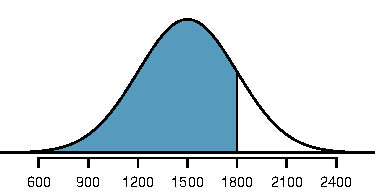
\includegraphics[height=1.5in]{ch_distributions/figures/satBelow1800/satBelow1800}
   \caption{The normal model for SAT scores, shading the area of those individuals who scored below Ann.}
   \label{satBelow1800}
\end{figure}

We can use the normal model to find percentiles. A \term{normal probability table}, which lists Z-scores and corresponding percentiles, can be used to identify a percentile based on the Z-score (and vice versa). Statistical software can also be used.

A normal probability table is given in Appendix~\vref{normalProbabilityTable} and abbreviated in Table~\ref{zTableShort}. We use this table to identify the percentile corresponding to any particular Z-score. For instance, the percentile of $Z=0.43$ is shown in row $0.4$ and column $0.03$ in Table~\ref{zTableShort}: 0.6664, or the $66.64^{th}$ percentile. Generally, we round $Z$ to two decimals, identify the proper row in the normal probability table up through the first decimal, and then determine the column representing the second decimal value. The intersection of this row and column is the percentile of the observation.

\begin{figure}
\centering
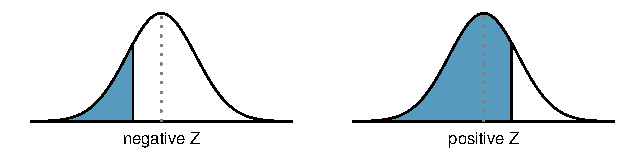
\includegraphics[width=0.9\textwidth]{ch_distributions/figures/normalTails/normalTails}
\caption{The area to the left of $Z$ represents the percentile of the observation.}
\label{normalTails}
\end{figure}

\begin{table}
\centering
\begin{tabular}{c | rrrrr | rrrrr |}
  \cline{2-11}
&&&& \multicolumn{4}{c}{Second decimal place of $Z$} &&& \\
  \cline{2-11}
$Z$ & 0.00 & 0.01 & 0.02 & \highlightT{0.03} & \highlightO{0.04} & 0.05 & 0.06 & 0.07 & 0.08 & 0.09 \\
  \hline
  \hline
0.0 & \scriptsize{0.5000} & \scriptsize{0.5040} & \scriptsize{0.5080} & \scriptsize{0.5120} & \scriptsize{0.5160} & \scriptsize{0.5199} & \scriptsize{0.5239} & \scriptsize{0.5279} & \scriptsize{0.5319} & \scriptsize{0.5359} \\
  0.1 & \scriptsize{0.5398} & \scriptsize{0.5438} & \scriptsize{0.5478} & \scriptsize{0.5517} & \scriptsize{0.5557} & \scriptsize{0.5596} & \scriptsize{0.5636} & \scriptsize{0.5675} & \scriptsize{0.5714} & \scriptsize{0.5753} \\
  0.2 & \scriptsize{0.5793} & \scriptsize{0.5832} & \scriptsize{0.5871} & \scriptsize{0.5910} & \scriptsize{0.5948} & \scriptsize{0.5987} & \scriptsize{0.6026} & \scriptsize{0.6064} & \scriptsize{0.6103} & \scriptsize{0.6141} \\
%  May comment out 0.0-0.2 to make extra space. Then insert the following line:
%  $\vdots$ &   $\vdots$ &   $\vdots$ &   $\vdots$ &   $\vdots$ &   $\vdots$ &   $\vdots$ &   $\vdots$ &   $\vdots$ &   $\vdots$ &   $\vdots$ \\
  0.3 & \scriptsize{0.6179} & \scriptsize{0.6217} & \scriptsize{0.6255} & \scriptsize{0.6293} & \scriptsize{0.6331} & \scriptsize{0.6368} & \scriptsize{0.6406} & \scriptsize{0.6443} & \scriptsize{0.6480} & \scriptsize{0.6517} \\
\highlightT{0.4} & \scriptsize{0.6554} & \scriptsize{0.6591} & \scriptsize{0.6628} & \highlightT{\scriptsize{0.6664}} & \scriptsize{0.6700} & \scriptsize{0.6736} & \scriptsize{0.6772} & \scriptsize{0.6808} & \scriptsize{0.6844} & \scriptsize{0.6879} \\
  \hline
  0.5 & \scriptsize{0.6915} & \scriptsize{0.6950} & \scriptsize{0.6985} & \scriptsize{0.7019} & \scriptsize{0.7054} & \scriptsize{0.7088} & \scriptsize{0.7123} & \scriptsize{0.7157} & \scriptsize{0.7190} & \scriptsize{0.7224} \\
  0.6 & \scriptsize{0.7257} & \scriptsize{0.7291} & \scriptsize{0.7324} & \scriptsize{0.7357} & \scriptsize{0.7389} & \scriptsize{0.7422} & \scriptsize{0.7454} & \scriptsize{0.7486} & \scriptsize{0.7517} & \scriptsize{0.7549} \\
  0.7 & \scriptsize{0.7580} & \scriptsize{0.7611} & \scriptsize{0.7642} & \scriptsize{0.7673} & \scriptsize{0.7704} & \scriptsize{0.7734} & \scriptsize{0.7764} & \scriptsize{0.7794} & \scriptsize{0.7823} & \scriptsize{0.7852} \\
\highlightO{0.8} & \scriptsize{0.7881} & \scriptsize{0.7910} & \scriptsize{0.7939} & \scriptsize{0.7967} & \highlightO{\scriptsize{0.7995}} & \scriptsize{0.8023} & \scriptsize{0.8051} & \scriptsize{0.8078} & \scriptsize{0.8106} & \scriptsize{0.8133} \\
  0.9 & \scriptsize{0.8159} & \scriptsize{0.8186} & \scriptsize{0.8212} & \scriptsize{0.8238} & \scriptsize{0.8264} & \scriptsize{0.8289} & \scriptsize{0.8315} & \scriptsize{0.8340} & \scriptsize{0.8365} & \scriptsize{0.8389} \\
  \hline
  \hline
  1.0 & \scriptsize{0.8413} & \scriptsize{0.8438} & \scriptsize{0.8461} & \scriptsize{0.8485} & \scriptsize{0.8508} & \scriptsize{0.8531} & \scriptsize{0.8554} & \scriptsize{0.8577} & \scriptsize{0.8599} & \scriptsize{0.8621} \\
  1.1 & \scriptsize{0.8643} & \scriptsize{0.8665} & \scriptsize{0.8686} & \scriptsize{0.8708} & \scriptsize{0.8729} & \scriptsize{0.8749} & \scriptsize{0.8770} & \scriptsize{0.8790} & \scriptsize{0.8810} & \scriptsize{0.8830} \\
  $\vdots$ &   $\vdots$ &   $\vdots$ &   $\vdots$ &   $\vdots$ &   $\vdots$ &   $\vdots$ &   $\vdots$ &   $\vdots$ &   $\vdots$ &   $\vdots$ \\
   \hline
\end{tabular}
\caption{A section of the normal probability table. The percentile for a normal random variable with $Z=0.43$ has been \highlightT{highlighted}, and the percentile closest to 0.8000 has also been \highlightO{highlighted}.}
\label{zTableShort}
\end{table}

We can also find the Z-score associated with a percentile. For example, to identify Z for the $80^{th}$ percentile, we look for the value closest to 0.8000 in the middle portion of the table: 0.7995. We determine the Z-score for the $80^{th}$ percentile by combining the row and column Z values: 0.84.

\begin{exercisewrap}
\begin{nexercise}
Determine the proportion of SAT test takers who scored better than Ann on the SAT.\footnotemark
\end{nexercise}
\end{exercisewrap}
\footnotetext{If 84\% had lower scores than Ann, the proportion of people who had better scores must be 16\%. (Generally ties are ignored when the normal model, or any other continuous distribution, is used.)}

%%
%%
\subsection{Normal probability examples}

Cumulative SAT scores are approximated well by a normal model with mean 1500 and standard deviation 300.

\begin{examplewrap}
\begin{nexample}{What is the probability that a randomly selected SAT taker scores at least 1630 on the SAT?}\label{satAbove1630Exam}
The probability that a randomly selected SAT taker scores at least 1630 on the SAT is equivalent to the proportion of all SAT takers that score at least 1630 on the SAT. First, always draw and label a picture of the normal distribution. (Drawings need not be exact to be useful.) We are interested in the probability that a randomly selected score will be above 1630, so we shade this upper tail:
\begin{center}
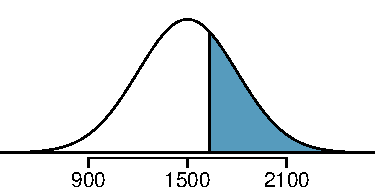
\includegraphics[height=0.9in]{ch_distributions/figures/satAbove1630/satAbove1630}
\end{center}
The picture shows the mean and the values at 2 standard deviations above and below the mean. The simplest way to find the shaded area under the curve makes use of the Z-score of the cutoff value. With $\mu=1500$, $\sigma=300$, and the cutoff value $x=1630$, the Z-score is computed as
\begin{eqnarray*}
Z = \frac{x - \mu}{\sigma} = \frac{1630 - 1500}{300} = \frac{130}{300} = 0.43
\end{eqnarray*}
We look up the percentile of $Z=0.43$ in the normal probability table shown in Table~\ref{zTableShort} or in Appendix~\vref{normalProbabilityTable}, which yields 0.6664. However, the percentile describes those who had a Z-score \emph{lower} than 0.43. To find the area \emph{above} $Z=0.43$, we compute one minus the area of the lower tail:
\begin{center}
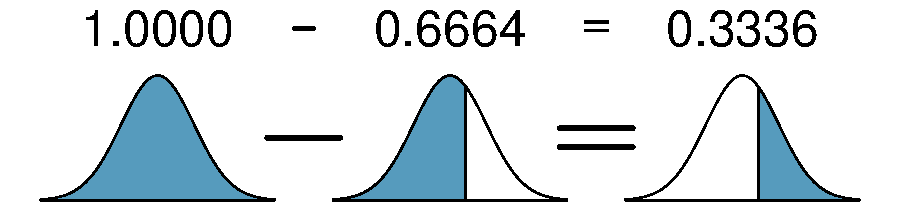
\includegraphics[height=0.8in]{ch_distributions/figures/subtractingArea/subtractingArea}
\end{center}
The probability that a randomly selected score is at least 1630 on the SAT is 0.3336.
\end{nexample}
\end{examplewrap}

\begin{onebox}{Always draw a picture first, and find the Z-score second}
For any normal probability situation, \emph{always always always} draw and label the normal curve and shade the area of interest first. The picture will provide an estimate of the probability. \vspace{3mm}

After drawing a figure to represent the situation, identify the Z-score for the observation of interest.\vspace{1mm}\end{onebox}

\begin{exercisewrap}
\begin{nexercise}
If the probability that a randomly selected score is at least 1630 is 0.3336, what is the probability that the score is less than 1630? Draw the normal curve representing this exercise, shading the lower region instead of the upper one.\footnotemark
\end{nexercise}
\end{exercisewrap}
\footnotetext{We found the probability in Example~\ref{satAbove1630Exam}: 0.6664. A picture for this exercise is represented by the shaded area below ``0.6664'' in Example~\ref{satAbove1630Exam}.}

\begin{examplewrap}
\begin{nexample}{Edward earned a 1400 on his SAT. What is his percentile?} \label{edwardSatBelow1400}
First, a picture is needed. Edward's percentile is the proportion of people who do not get as high as a 1400. These are the scores to the left of 1400.
\begin{center}
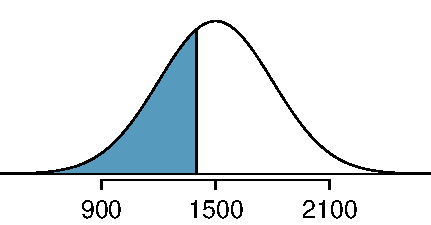
\includegraphics[height=22mm]{ch_distributions/figures/satBelow1400/satBelow1400}
\end{center}
Identifying the mean $\mu=1500$, the standard deviation $\sigma=300$, and the cutoff for the tail area $x=1400$ makes it easy to compute the Z-score:
\begin{eqnarray*}
Z = \frac{x - \mu}{\sigma} = \frac{1400 - 1500}{300} = -0.33
\end{eqnarray*}
Using the normal probability table, identify the row of $-0.3$ and column of $0.03$, which corresponds to the probability $0.3707$. Edward is at the $37^{th}$ percentile.
\end{nexample}
\end{examplewrap}

\begin{exercisewrap}
\begin{nexercise}
Use the results of Example~\ref{edwardSatBelow1400} to compute the proportion of SAT takers who did better than Edward. Also draw a new picture.\footnotemark
\end{nexercise}
\end{exercisewrap}
\footnotetext{If Edward did better than 37\% of SAT takers, then about 63\% must have done better than him. \\
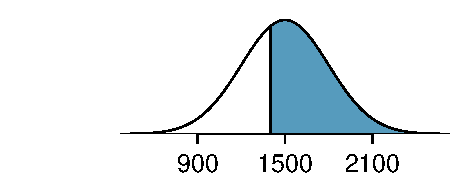
\includegraphics[height=12mm]{ch_distributions/figures/satBelow1400/satAbove1400}}


\begin{onebox}{Areas to the right}
The normal probability table in most books gives the area to the left. If you would like the area to the right, first find the area to the left and then subtract this amount from~one.\end{onebox}

The last several problems have focused on finding the probability or percentile for a particular observation. It is also possible to identify the value corresponding to a particular percentile.

\begin{examplewrap}
\begin{nexample}{Carlos believes he can get into his preferred college if he scores at least in the 80th percentile on the SAT. What score should he aim for?}
Here, we are given a percentile rather than a Z-score, so we work backwards. As always, first draw the picture.
\begin{center}
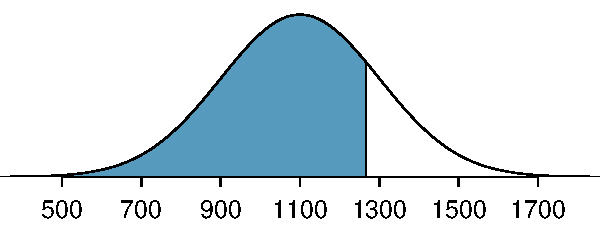
\includegraphics[height=22mm]{ch_distributions/figures/sat80thPercentile/sat80thPercentile}
\end{center}
We want to find the observation that corresponds to the 80th percentile. First, we find the Z-score associated with the 80th percentile using the normal probability table. Looking at Table~\ref{zTableShort}., we look for the number closest to 0.80 \emph{inside} the table. The closest number we find is 0.7995 (highlighted). 0.7995 falls on row 0.8 and column 0.04, therefore it corresponds to a Z-score of 0.84. In any normal distribution, a value with a Z-score of 0.84 will be at the 80th percentile. Once we have the Z-score, we work backwards to find x.
\begin{align*}
Z &= \frac{x-\mu}{\sigma} \\
0.84 &= \frac{x-1500}{300} \\
0.84 \times 300+1500 &= x \\
x& = 1752
\end{align*}
The 80th percentile on the SAT corresponds to a score of 1752.
\end{nexample}
\end{examplewrap}

\begin{exercisewrap}
\begin{nexercise}Imani scored at the 72nd percentile on the SAT. What was her SAT score?\footnotemark\end{nexercise}
\end{exercisewrap}
\footnotetext{First, draw a picture! The closest percentile in the table to 0.72 is 0.7190, which corresponds to $Z = 0.58$. Next, set up the Z-score formula and solve for $x$: $0.58 = \frac{x-1500}{300} \rightarrow x = 1674$. Imani scored 1674.}


\begin{onebox}{If the data are not nearly normal, don't use a normal table}
{Before using the normal table, verify that the data or distribution is approximately normal. If it is not, the normal table will give incorrect results. Also, all answers based on normal approximations are approximations and are not exact.}
\end{onebox}



%%
%%
\subsection{Calculator: finding normal probabilities}
\label{normal}

\begin{onebox}{\videohref{ti84_normal_curve_area} TI-84: Finding area under the normal curve}
Use \calcbutton{2ND} \calcbutton{VARS}, \calctext{normalcdf} to find an area/proportion/probability between two Z-scores or to the left or right of a Z-score.\vspace{-1mm}
\begin{enumerate}
\setlength{\itemsep}{0mm}
\item Choose \calcbutton{2ND} \calcbutton{VARS} (i.e. \calctext{DISTR}).
\item Choose \calctext{2:normalcdf}.
\item Enter the \calctext{lower} (left) Z-score and the \calctext{upper} (right) Z-score.
\vspace{-1.5mm}
  \begin{itemize}
  \setlength{\itemsep}{0mm}
  \item If finding just a lower tail area, set \calctext{lower} to \calctext{-5}.
  \item If finding just an upper tail area, set \calctext{upper} to \calctext{5}.
\end{itemize}
\item Leave $\calctextmath{\mu}$ as \calctext{0} and $\calctextmath{\sigma}$ as \calctext{1}.
\item Down arrow, choose \calctext{Paste}, and hit \calcbutton{ENTER}.\vspace{-1.5mm}
\end{enumerate}
TI-83: Do steps 1-2, then enter the lower bound and upper bound separated by a comma, e.g. \calctext{normalcdf(2, 5)}, and hit \calcbutton{ENTER}.\end{onebox}

\begin{onebox}[]{\videohref{casio_normal_curve_area} Casio fx-9750GII: Finding area under the normal curve}
\begin{enumerate}
\setlength{\itemsep}{0mm}
\item Navigate to \calctext{STAT} (\calcbutton{MENU}, then hit \calcbutton{2}).
\item Select \calctext{DIST} (\calcbutton{F5}), then \calctext{NORM} (\calcbutton{F1}), and then \calctext{Ncd} (\calcbutton{F2}).
\item If needed, set \calctext{Data} to \calctext{Variable} (\calctext{Var} option, which is \calcbutton{F2}).
\item Enter the \calctext{Lower} Z-score and the \calctext{Upper} Z-score. Set $\calctextmath{\sigma}$ to \calctext{1} and $\calctextmath{\mu}$ to \calctext{0}.\vspace{-1.5mm}
  \begin{itemize}
  \setlength{\itemsep}{0mm}
  \item If finding just a lower tail area, set \calctext{Lower} to \calctext{-5}.
  \item For an upper tail area, set \calctext{Upper} to \calctext{5}.
  %\item If finding a middle area (e.g. $Z_{lower} = 0.5$ to $Z_{upper} = 1.5$), set the \calctext{lower} and \calctext{upper} values appropriately.
  \end{itemize}
\item Hit \calctext{EXE}, which will return the area probability (\calctext{p}) along with the Z-scores for the lower and upper bounds.
\end{enumerate}
\end{onebox}

\begin{examplewrap}
\begin{nexample}{Use a calculator to determine what percentile corresponds to a Z-score of 1.5.}
Always first sketch a graph:\footnotemark
\begin{center}
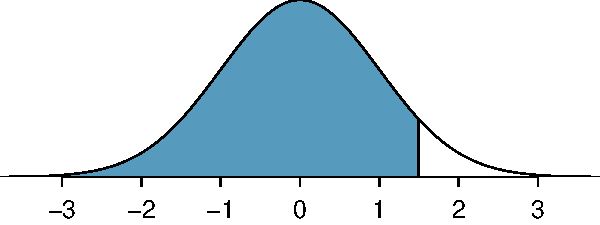
\includegraphics[width=0.57\textwidth]{ch_distributions/figures/zscoreleftof1point5/zscoreleftof1point5}\vspace{-2mm}
\end{center}
To find an area under the normal curve using a calculator, first identify a lower bound and an upper bound. Theoretically, we want all of the area to the left of 1.5, so the left endpoint should be -$\infty$. However, the area under the curve is nearly negligible when $Z$ is smaller than -4, so we will use -5 as the lower bound when not given a lower bound (any other negative number smaller than -5 will also work). Using a lower bound of -5 and an upper bound of 1.5, we get $P(Z < 1.5) = 0.933$.
\end{nexample}
\end{examplewrap}
\footnotetext{normalcdf gives the result without drawing the graph. To draw the graph, do 2nd VARS, DRAW, 1:ShadeNorm. However, beware of errors caused by other plots that might interfere with this plot.}

\begin{exercisewrap}
\begin{nexercise}
Find the area under the normal curve to right of $Z=2$.~\footnotemark
\end{nexercise}
\end{exercisewrap}
\footnotetext{Now we want to shade to the right. Therefore our lower bound will be 2 and the upper bound will be +5 (or a number bigger than 5) to get $P(Z > 2) = 0.023$.}

\begin{exercisewrap}
\begin{nexercise}Find the area under the normal curve between -1.5 and~1.5.~\footnotemark\end{nexercise}
\end{exercisewrap}
\footnotetext{Here we are given both the lower and the upper bound. Lower bound is -1.5 and upper bound is 1.5. The area under the normal curve between -1.5 and 1.5 = $P(-1.5 < Z < 1.5) = 0.866$.}


\begin{onebox}{\videohref{ti84_Z_score_for_a_percentile} TI-84: Find a Z-score that corresponds to a percentile}
\label{invNorm}
Use \calcbutton{2ND} \calcbutton{VARS}, \calctext{invNorm} to find the Z-score that corresponds to a given percentile.
\begin{enumerate}
\setlength{\itemsep}{0mm}
\item Choose \calcbutton{2ND} \calcbutton{VARS} (i.e. \calctext{DISTR}).
\item Choose \calctext{3:invNorm}.
\item Let \calctext{Area} be the percentile as a decimal (the area to the left of desired Z-score).
\item Leave $\calctextmath{\mu}$ as \calctext{0} and $\calctextmath{\sigma}$ as \calctext{1}.
\item Down arrow, choose \calctext{Paste}, and hit \calcbutton{ENTER}.\vspace{-1.5mm}
\end{enumerate}
TI-83: Do steps 1-2, then enter the percentile as a decimal, e.g.~\mbox{\calctext{invNorm(.40)},} then hit \calcbutton{ENTER}.\end{onebox}

\begin{onebox}[]{\videohref{casio_Z_score_for_a_percentile} Casio fx-9750GII: Find a Z-score that corresponds to a percentile}
\begin{enumerate}
\setlength{\itemsep}{0mm}
\setlength{\itemsep}{0mm}
\item Navigate to \calctext{STAT} (\calcbutton{MENU}, then hit \calcbutton{2}).
\item Select \calctext{DIST} (\calcbutton{F5}), then \calctext{NORM} (\calcbutton{F1}), and then \calctext{InvN} (\calcbutton{F3}).
\item If needed, set \calctext{Data} to \calctext{Variable} (\calctext{Var} option, which is \calcbutton{F2}).
\item Decide which tail area to use (\calctext{Tail}), the tail area (\calctext{Area}), and then enter the $\calctextmath{\sigma}$ and $\calctextmath{\mu}$ values.
\item Hit \calctext{EXE}.
\end{enumerate}
\end{onebox}

\begin{examplewrap}
\begin{nexample}{Use a calculator to find the Z-score that corresponds to the 40th percentile.}Letting Area be 0.40, a calculator gives -0.253. This means that $Z = -0.253$ corresponds to the 40th percentile, that~is, $P(Z < -0.253) = 0.40$.
\end{nexample}
\end{examplewrap}

\begin{exercisewrap}
\begin{nexercise}Find the Z-score such that 20 percent of the area is to the right of that Z-score.\footnotemark\end{nexercise}
\end{exercisewrap}	
\footnotetext{If 20\% of the area is the right, then 80\% of the area is to the left. Letting area be 0.80, we get $Z = 0.841$.}


\begin{examplewrap}
\begin{nexample}{In a large study of birth weight of newborns, the weights of 23,419 newborn boys were recorded.\footnotemark\, The distribution of weights was approximately normal with a mean of 7.44 lbs (3376 grams) and a standard deviation of 1.33 lbs (603 grams). The government classifies a newborn as having low birth weight if the weight is less than 5.5 pounds. What percent of these newborns had a low birth weight?}
We find an area under the normal curve between -5 (or a number smaller than -5, e.g. -10) and a Z-score that we will calculate. There is no need to write calculator commands in a solution. Instead, continue to use standard statistical notation. 
\begin{align*}
Z&=\frac{5.5-7.44}{1.33}\\
&=-1.49\\
P(Z < -1.49) &= 0.068
\end{align*}
Approximately 6.8\% of the newborns were of low birth weight.
\end{nexample}
\end{examplewrap}
\footnotetext{\oiRedirect{textbook-birthweight_for_Scottish_singleton_births}{www.biomedcentral.com/1471-2393/8/5}}

\begin{exercisewrap}
\begin{nexercise}Approximately what percent of these babies weighed greater than 10 pounds?\footnotemark\end{nexercise}
\end{exercisewrap}
\footnotetext{$Z=\frac{10-7.44}{1.33}=1.925$. Using a lower bound of 2 and an upper bound of 5, we get $P(Z > 1.925) = 0.027$. Approximately 2.7\% of the newborns weighed over 10 pounds.}


\begin{exercisewrap}
\begin{nexercise}Approximately \emph{how many} of these newborns weighed greater than 10 pounds?\footnotemark
\end{nexercise}
\end{exercisewrap}
\footnotetext{Approximately 2.7\% of the newborns weighed over 10 pounds. Because there were 23,419 of them, about $0.027 \times 23419 \approx 632$ weighed greater than 10 pounds.}

\begin{exercisewrap}
\begin{nexercise}How much would a newborn have to weigh in order to be at the 90th percentile among this group?\footnotemark
\end{nexercise}
\end{exercisewrap}
\footnotetext{Because we have the percentile, this is the inverse problem. To get the Z-score, use the inverse normal option with 0.90 to get $Z = 1.28$. Then solve for $x$ in $1.28 = \frac{x - 7.44}{1.33}$ to get $x = 9.15$. To be at the 90th percentile among this group, a newborn would have to weigh 9.15 pounds.}

%%
%%
\subsection{68-95-99.7 rule}

Here, we present a useful rule of thumb for the probability of falling within 1, 2, and 3 standard deviations of the mean in the normal distribution. This will be useful in a wide range of practical settings, especially when trying to make a quick estimate without a calculator or Z table.

\begin{figure}[hht]
\centering
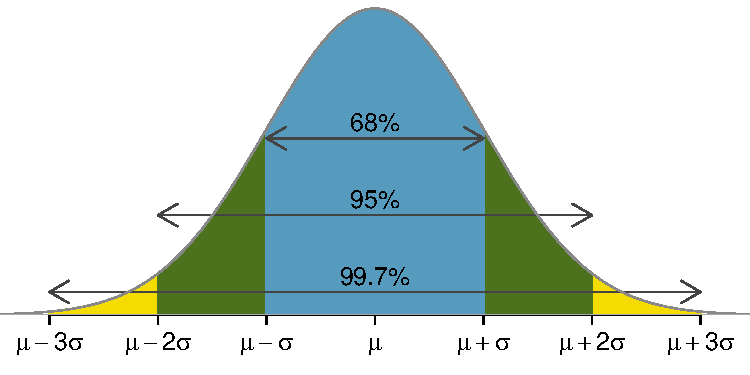
\includegraphics[width=0.78\textwidth]{ch_distributions/figures/6895997/6895997}
\caption{Probabilities for falling within 1, 2, and 3 standard deviations of the mean in a normal distribution.}
\label{6895997}
\end{figure}

\begin{exercisewrap}
\begin{nexercise}
Use the Z table to confirm that about 68\%, 95\%, and 99.7\% of observations fall within 1, 2, and 3, standard deviations of the mean in the normal distribution, respectively. For instance, first find the area that falls between $Z=-1$ and $Z=1$, which should have an area of about 0.68. Similarly there should be an area of about 0.95 between $Z=-2$ and $Z=2$.\footnotemark\end{nexercise}
\end{exercisewrap}
\footnotetext{First draw the pictures. To find the area between $Z=-1$ and $Z=1$, use the normal probability table to determine the areas below $Z=-1$ and above $Z=1$. Next verify the area between $Z=-1$ and $Z=1$ is about 0.68. Repeat this for $Z=-2$ to $Z=2$ and also for $Z=-3$ to $Z=3$.}


It is possible for a normal random variable to fall 4,~5, or~even more standard deviations from the mean. However, these occurrences are very rare if the data are nearly normal. The probability of being further than 4 standard deviations from the mean is about 1-in-15,000. For 5 and 6 standard deviations, it is about 1-in-2 million and 1-in-500 million, respectively.

\begin{exercisewrap}
\begin{nexercise}
SAT scores closely follow the normal model with mean $\mu = 1500$ and standard deviation $\sigma = 300$. (a) About what percent of test takers score 900 to 2100? (b) What percent score between 1500 and 2100?\footnotemark
\end{nexercise}
\end{exercisewrap}
\footnotetext{(a) 900 and 2100 represent two standard deviations above and below the mean, which means about 95\% of test takers will score between 900 and 2100. (b)~Since the normal model is symmetric, then half of the test takers from part~(a) ($\frac{95\%}{2} = 47.5\%$ of all test takers) will score 900 to 1500 while 47.5\% score between 1500 and 2100.}

%%
%%
\subsection{Evaluating the normal approximation}
\label{assessingNormal}

It is important to remember normality is always an approximation. Testing the appropriateness of the normal assumption is a key step in many data analyses.

\index{normal probability plot|(}

The distribution of heights of US males is well approximated by the normal model. We are interested in proceeding under the assumption that the data are normally distributed, but first we must check to see if this is reasonable.

There are two visual methods for checking the assumption of normality that can be implemented and interpreted quickly. The first is a simple histogram with the best fitting normal curve overlaid on the plot, as shown in the left panel of Figure~\ref{fcidMHeights}. The sample mean $\bar{x}$ and standard deviation $s$ are used as the parameters of the best fitting normal curve. The closer this curve fits the histogram, the more reasonable the normal model assumption. Another more common method is examining a \term{normal probability plot},\footnote{Also commonly called a \term{quantile-quantile plot}.} shown in the right panel of Figure~\ref{fcidMHeights}. The closer the points are to a perfect straight line, the more confident we can be that the data follow the normal model.

\begin{figure}[ht]
\centering
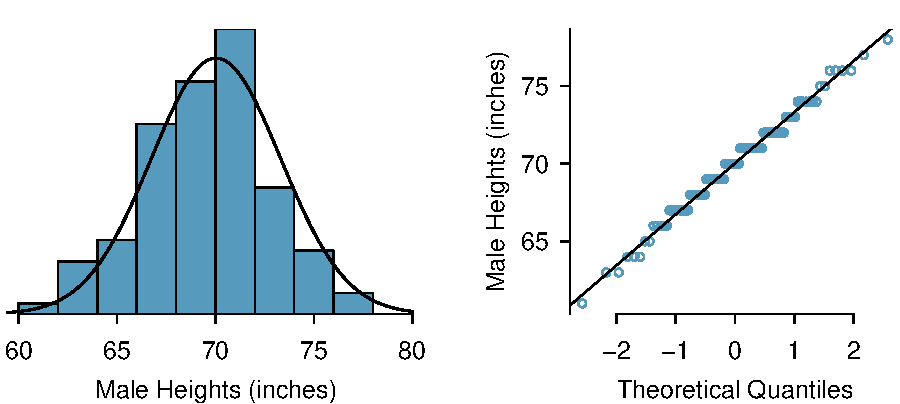
\includegraphics[width=0.78\textwidth]{ch_distributions/figures/fcidMHeights/fcidMHeights}
\caption{A sample of 100 male heights. The observations are rounded to the nearest whole inch, explaining why the points appear to jump in increments in the normal probability plot.}
\label{fcidMHeights}
\end{figure}

\textA{\pagebreak}

Three data sets of 40, 100, and 400 samples were simulated from a normal distribution, and the histograms and normal probability plots of the data sets are shown in Figure~\ref{normalExamples}. These will provide a benchmark for what to look for in plots of real data. \label{normalExamplesExample}

\begin{figure}
\centering
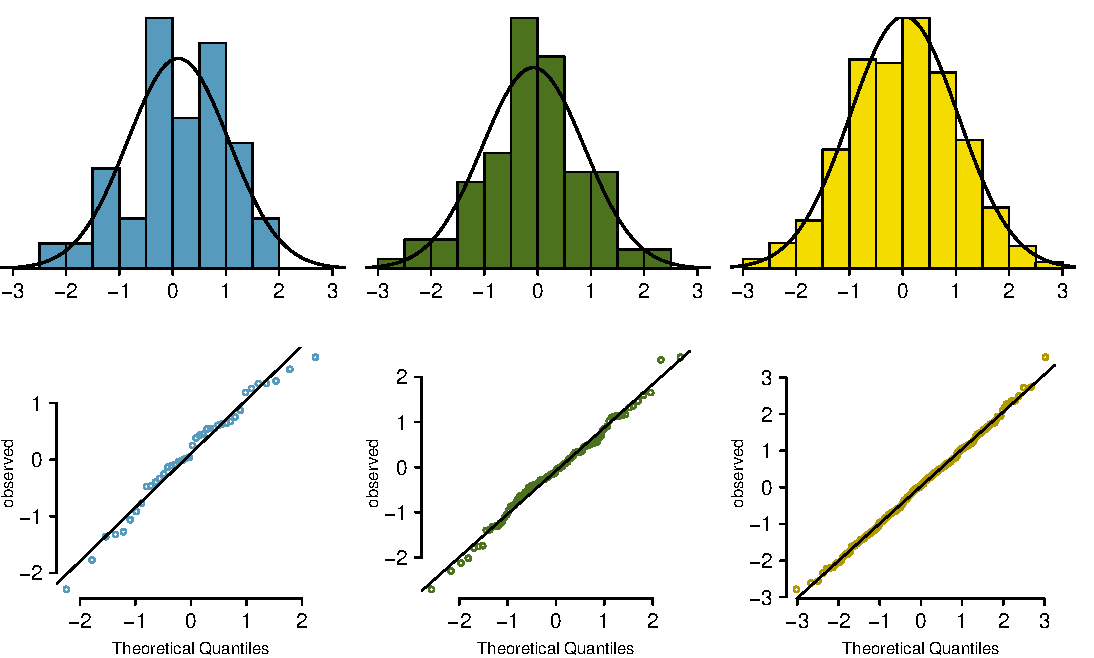
\includegraphics[width=\textwidth]{ch_distributions/figures/normalExamples/normalExamples}
\caption{Histograms and normal probability plots for three simulated normal data sets; $n=40$ (left), $n=100$ (middle), $n=400$ (right).}
\label{normalExamples}
\end{figure}

The left panels show the histogram (top) and normal probability plot (bottom) for the simulated data set with 40 observations. The data set is too small to really see clear structure in the histogram. The normal probability plot also reflects this, where there are some deviations from the line. However, these deviations are not strong.

The middle panels show diagnostic plots for the data set with 100 simulated observations. The histogram shows more normality and the normal probability plot shows a better fit. While there is one observation that deviates noticeably from the line, it is not particularly extreme.

The data set with 400 observations has a histogram that greatly resembles the normal distribution, while the normal probability plot is nearly a perfect straight line. Again in the normal probability plot there is one observation (the largest) that deviates slightly from the line. If that observation had deviated 3 times further from the line, it would be of much greater concern in a real data set. Apparent outliers can occur in normally distributed data but they are rare.

Notice the histograms look more normal as the sample size increases, and the normal probability plot becomes straighter and more stable.


\begin{examplewrap}
\begin{nexample}{Are NBA player heights normally distributed? Consider all 435 NBA players from the 2008-9 season presented in Figure~\ref{nbaNormal}.\footnotemark\, We first create a histogram and normal probability plot of the NBA player heights. The histogram in the left panel is slightly left skewed, which contrasts with the symmetric normal distribution. The points in the normal probability plot do not appear to closely follow a straight line but show what appears to be a ``wave''. We can compare these characteristics to the sample of 400 normally distributed observations in Example~\ref{normalExamplesExample} and see that they represent much stronger deviations from the normal model. NBA player heights do not appear to come from a normal distribution.
\end{nexample}
\end{examplewrap}
\footnotetext{These data were collected from \oiRedirect{textbook-nba_com}{www.nba.com}.}}

\begin{figure}
\centering
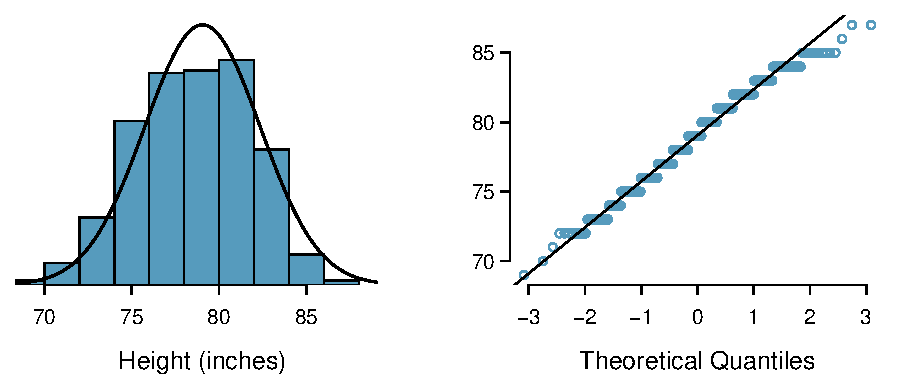
\includegraphics[width=\textwidth]{ch_distributions/figures/nbaNormal/nbaNormal}
\caption{Histogram and normal probability plot for the NBA heights from the 2008-9 season.}
\label{nbaNormal}
\end{figure}

\begin{examplewrap}
\begin{nexample}{Can we approximate poker winnings by a normal distribution? We consider the poker winnings of an individual over 50 days. A histogram and normal probability plot of these data are shown in Figure~\ref{pokerNormal}.}
The data are very strongly right skewed\index{skew!example: very strong} in the histogram, which corresponds to the very strong deviations on the upper right component of the normal probability plot. If we compare these results to the sample of 40 normal observations in Example~\ref{normalExamplesExample}, it is apparent that these data show very strong deviations from the normal model.
\end{nexample}
\end{examplewrap}

\begin{figure}
\centering
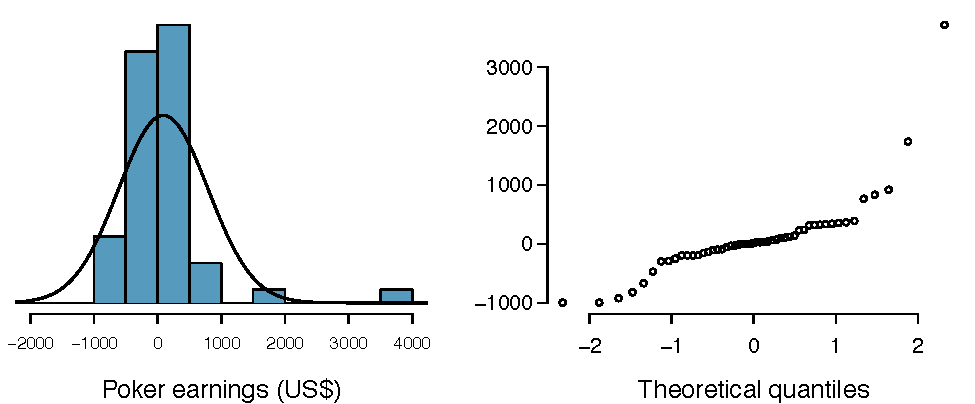
\includegraphics[width=\textwidth]{ch_distributions/figures/pokerNormal/pokerNormal}
\caption{A histogram of poker data with the best fitting normal plot and a normal probability plot.}
\label{pokerNormal}
\end{figure}

\begin{exercisewrap}
\begin{nexercise}\label{normalQuantileExercise}
Determine which data sets represented in Figure~\ref{normalQuantileExer} plausibly come from a nearly normal distribution. Are you confident in all of your conclusions? There are 100 (top left), 50 (top right), 500 (bottom left), and 15 points (bottom right) in the four plots.\footnotemark
\end{nexercise}
\end{exercisewrap}
\footnotetext{Answers may vary a little. The top-left plot shows some deviations in the smallest values in the data set; specifically, the left tail of the data set has some outliers we should be wary of. The top-right and bottom-left plots do not show any obvious or extreme deviations from the lines for their respective sample sizes, so a normal model would be reasonable for these data sets. The bottom-right plot has a consistent curvature that suggests it is not from the normal distribution. If we examine just the vertical coordinates of these observations, we see that there is a lot of data between -20 and 0, and then about five observations scattered between 0 and 70. This describes a distribution that has a strong right skew.}

\begin{figure}
\centering
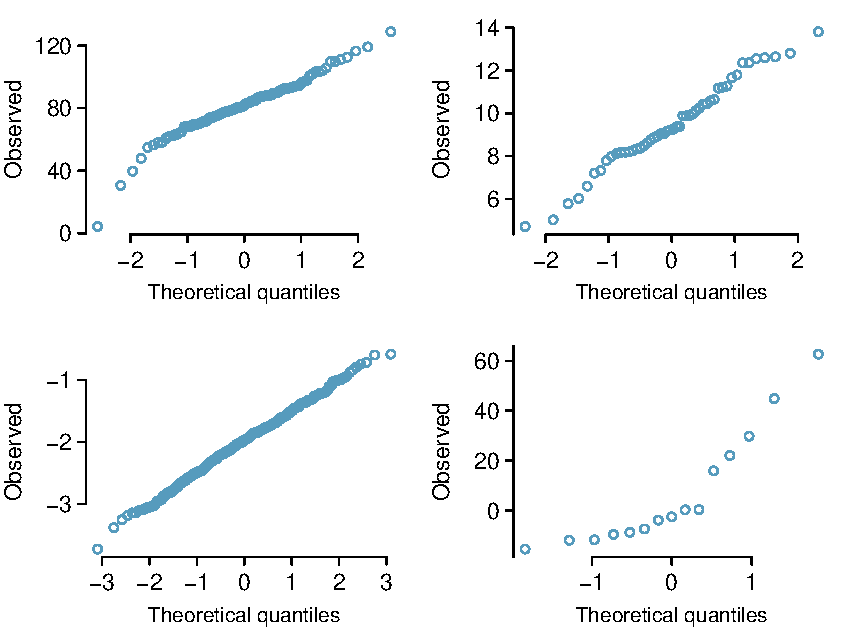
\includegraphics[width=0.9\textwidth]{ch_distributions/figures/normalQuantileExer/normalQuantileExer}
\caption{Four normal probability plots for Guided Practice~\ref{normalQuantileExercise}.}
\label{normalQuantileExer}
\end{figure}

\begin{exercisewrap}
\begin{nexercise} \label{normalQuantileExerciseAdditional}
Figure~\ref{normalQuantileExerAdditional} shows normal probability plots for two distributions that are skewed. One distribution is skewed to the low end (left skewed) and the other to the high end (right skewed). Which is which?\footnotemark
\end{nexercise}
\end{exercisewrap}
\footnotetext{Examine where the points fall along the vertical axis. In the first plot, most points are near the low end with fewer observations scattered along the high end; this describes a distribution that is skewed to the high end. The second plot shows the opposite features, and this distribution is skewed to the low end.}


\begin{figure}
\centering
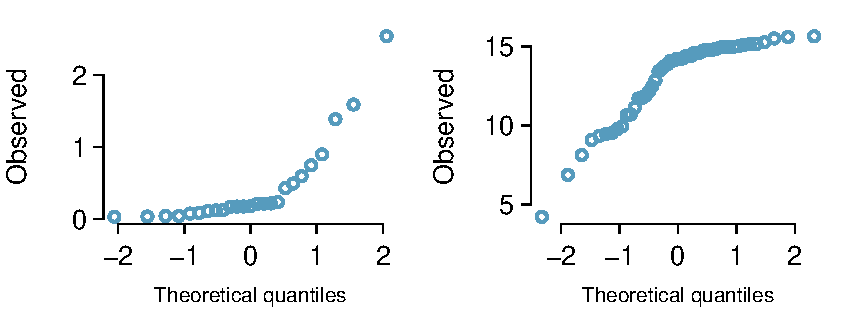
\includegraphics[width=0.9\textwidth]{ch_distributions/figures/normalQuantileExer/normalQuantileExerAdditional}
\caption{Normal probability plots for Guided Practice~\ref{normalQuantileExerciseAdditional}.}
\label{normalQuantileExerAdditional}
\end{figure}


%%
%%
\subsection{Normal approximation for sums of random variables}
\label{normapproxsumrv}

\Comment{check on text break past images on next page}

We have seen that many distributions are approximately normal. The sum and the difference of normally distributed variables is also normal. While we cannot prove this here, the usefulness of it is seen in the following example.

\begin{examplewrap}
\begin{nexample}{Three friends are playing a cooperative video game in which they have to complete a puzzle as fast as possible. Assume that the individual times of the 3 friends are independent of each other. The individual times of the friends in similar puzzles are approximately normally distributed with the following means and standard deviations. 
\begin{center}
\begin{tabular}{lrr}
& Mean &  SD \\
Friend 1 	& 5.6 & 0.11  \\
Friend 2 	& 5.8  & 0.13 \\
Friend 3 	& 6.1  & 0.12  
\end{tabular}
\end{center}
To advance to the next level of the game, the friends' total time must not exceed 17.1 minutes. What is the probability that they will advance to the next level?}
Because each friend's time is approximately normally distributed, \emph{the sum of their times is also approximately normally distributed}. We will do a normal approximation, but first we need to find the mean and standard deviation of the \emph{sum}. We learned how to do this in Section~\ref{randomVariablesSection}.

Let the three friends be labeled $X$, $Y$, $Z$. We want $P(X + Y + Z < 17.1)$. The mean and standard deviation of the sum of $X$, $Y$, and $Z$ is given by:
\begin{align*}
\mu_{sum} &= E(X+Y+Z)
	& \sigma_{sum}&= \sqrt{(SD_X)^2+(SD_Y)^2 + (SD_Z)^2} \\
&= E(X) + E(Y) + E(Z)
	& &= \sqrt{(0.11)^2+(0.13)^2+(0.12)^2}\\
&=4.6+4.8+4.5
	& &= 0.208 \\
&=17.5
\end{align*}
Now we can find the Z-score. 
\begin{align*}
Z &= \frac{x_{sum}-\mu_{sum}}{\sigma_{sum}} \\
&=\frac{17.1-17.5}{0.208} \\
&=-1.92
\end{align*}
Finally, we want the probability that the sum is less than 17.5, so we shade the area to the left of $Z = -1.92$. Using the normal table or a calculator, we get
\begin{align*}
P(Z < -1.92) = 0.027
\end{align*}
There is a 2.7\% chance that the friends will advance to the next level.
\end{nexample}
\end{examplewrap}

\begin{exercisewrap}
\begin{nexercise}
What is the probability that Friend 2 will complete the puzzle with a faster time than Friend 1?  Hint:  find $P(Y < X)$, or $P(Y - X < 0)$.\footnotemark
\end{nexercise}
\end{exercisewrap}
\footnotetext{First find the mean and standard deviation of $Y - X$. The mean of $Y - X$ is $\mu_{Y-X} = 5.8 - 5.6 =  0.2$. The standard deviation is  $SD_{Y-X}=\sqrt{(0.13)^2+(0.11)^2}=0.170$. Then $Z=\frac{0-0.2}{0.170}=-1.18$ and $P(Z < -1.18)= .119$. There is an 11.9\% chance that Friend 2 will complete the puzzle with a faster time than Friend 1.}

%%
%%
\subsection*{Section summary}

\begin{itemize}
\item A \term{Z-score} represents the number of standard deviations a value in a data set is above or below the mean.  To calculate a \mbox{Z-score} use: $Z = \frac{x-\text{mean}}{SD}$.  

\item \emph{Z-scores do not depend on units}.  When looking at distributions with different units or different standard deviations, \mbox{Z-scores} are useful for comparing how far values are away from the mean (relative to the distribution of the data). 

\item The \term{normal distribution} is the most commonly used distribution in Statistics.  Many distribution are approximately normal, but none are exactly normal.  

\item The \term{68-95-99.7 Rule}, otherwise known as the empirical rule, comes from the normal distribution.  The closer a distribution is to normal, the better this rule will hold.

\item It is often useful to use the standard normal distribution, which has mean~0 and SD~1, to approximate a discrete histogram.  There are two common types of \textbf{normal approximation problems}, and for each a key step is to find a \mbox{Z-score}.   
\begin{itemize}
\item[A:] \textit{Find the percent or probability of a value greater/less than a given \textit{x}-value.  }
\begin{enumerate}\vspace{-1mm}
\setlength{\itemsep}{0mm}
\item Verify that the distribution of interest is approximately normal.
\item Calculate the \mbox{Z-score}.  Use the provided population mean and SD to standardize the given $x$-value.
\item Use a calculator function (e.g. \calctext{normcdf} on a TI) or a normal table to find the area under the normal curve to the right/left of this \mbox{Z-score}; this is the \textit{estimate} for the percent/probability.
\end{enumerate}

\item[B:] \textit{Find the \textit{x}-value that corresponds to a given percentile.}
\begin{enumerate}\vspace{-1mm}
\setlength{\itemsep}{0mm}
\item Verify that the distribution of interest is approximately normal.
\item Find the Z-score that corresponds to the given percentile (using, for example, \calctext{invNorm} on a TI).  
\item Use the Z-score along with the given mean and SD to solve for the \textit{x}-value.  
\end{enumerate}
\end{itemize}

\item Because the sum or difference of two normally distributed variables is itself a normally distributed variable, the normal approximation is also used in the following type of problem.
\item[] \textit{Find the probability that a sum $X+Y$ or a difference $X-Y$ is greater/less than some value}.
\begin{enumerate}\vspace{-1mm}
\setlength{\itemsep}{0mm}
\item Verify that the distribution of $X$ and the distribution of $Y$ are approximately normal.  
\item Find the mean of the sum or difference.  Recall: the mean of a sum is the 
\\sum of the means.  The mean of a difference is the difference of the means.  
\\Find the SD of the sum or difference using:  
\\$SD(X+Y) = SD(X - Y) =  \sqrt{(SD(X))^2 + (SD(Y))^2}$.
\item Calculate the Z-score.  Use the calculated mean and SD to standardize the given sum or difference.
\item Find the appropriate area under the normal curve. 
\end{enumerate}


\end{itemize}

%____________________________________
\section[Sampling distribution of a sample mean]{Sampling distribution of a sample mean }
\label{distributionofxbar}

\sectionintro{

%%
\subsection*{Learning objectives}
\begin{enumerate}
\item Understand the concept of a sampling distribution.

\item Describe the center, spread, and shape of the sampling distribution of a sample mean.


\item Distinguish between the standard deviation of a population and the standard deviation of a sampling distribution.

\item Explain the content and importance of the Central Limit Theorem.

\item Identify and explain the conditions for using normal approximation involving a sample mean.

\item Verify that the conditions for normal approximation are met and carry out normal approximation involving a sample mean or sample sum.

\end{enumerate}
}


%%
\subsection{The mean and standard deviation of $\bar{x}$}


In this section we consider a data set called \data{run10}, which represents all 16,924 runners who finished the 2012 Cherry Blossom 10 mile run in Washington, DC.\footnote{\oiRedirect{textbook-cherryblossom_org}{www.cherryblossom.org}} Part of this data set is shown in Table~\ref{run10DF}, and the variables are described in Table~\ref{run10Variables}.

\begin{table}[h]
\centering
\begin{tabular}{rrrrr}
  \hline
ID & time & age & gender & state \\ 
  \hline
1 & 92.25 & 38.00 & M & MD \\ 
2 & 106.35 & 33.00 & M & DC \\ 
3 & 89.33 & 55.00 & F & VA \\ 
4 & 113.50 & 24.00 & F & VA \\ 
$\vdots$ & $\vdots$ & $\vdots$ & $\vdots$ & $\vdots$ \\
16923 & 122.87 & 37.00 & F & VA \\ 
16924 & 93.30 & 27.00 & F & DC \\ 
   \hline
\end{tabular}
\caption{Six observations from the \data{run10} data set.}
\label{run10DF}
\end{table}
% library(openintro); library(xtable); data(run10); xtable(run10[c(1,2,3,4, nrow(run10)-1:0), c("time", "age", "gender", "state")])

\begin{table}[h]
\centering\small
\begin{tabular}{l p{65mm}}
\hline
{\bf variable} & {\bf description} \\
\hline
\var{time} & Ten mile run time, in minutes \\
\var{age} & Age, in years \\
\var{gender} & Gender (\resp{M} for male, \resp{F} for female) \\
\var{state} & Home state (or country if not from the US) \\
\hline
\end{tabular}
\caption{Variables and their descriptions for the \data{run10} data set.}
\label{run10Variables}
\end{table}

\index{data!run10Samp|(}

These data are special because they include the results for the entire population of runners who finished the 2012 Cherry Blossom Run. We took a simple random sample of this population, which is represented in Table~\ref{run10SampDF}. A histogram summarizing the time variable in the \data{run10Samp} data set is shown in Figure~\ref{run10SampHistograms}.

\begin{table}
\centering
\begin{tabular}{rrrrr}
  \hline
ID & time & age & gender & state \\ 
  \hline
1983 & 88.31 & 59 & M & MD \\ 
8192 & 100.67 & 32 & M & VA \\ 
11020 & 109.52 & 33 & F & VA \\ 
  $\vdots$ &   $\vdots$ &   $\vdots$ &   $\vdots$ &   $\vdots$ \\ 
1287 & 89.49 & 26 & M & DC \\ 
   \hline
\end{tabular}
\caption{Four observations for the \data{run10Samp} data set, which represents a simple random sample of 100 runners from the 2012 Cherry Blossom Run.}
\label{run10SampDF}
%library(openintro); library(xtable); data(run10); data(run10Samp); xtable(run10Samp[c(1,2,3,100),])
\end{table}

% WARNING: This figure is referenced in Section 4.2

\begin{figure}
\centering
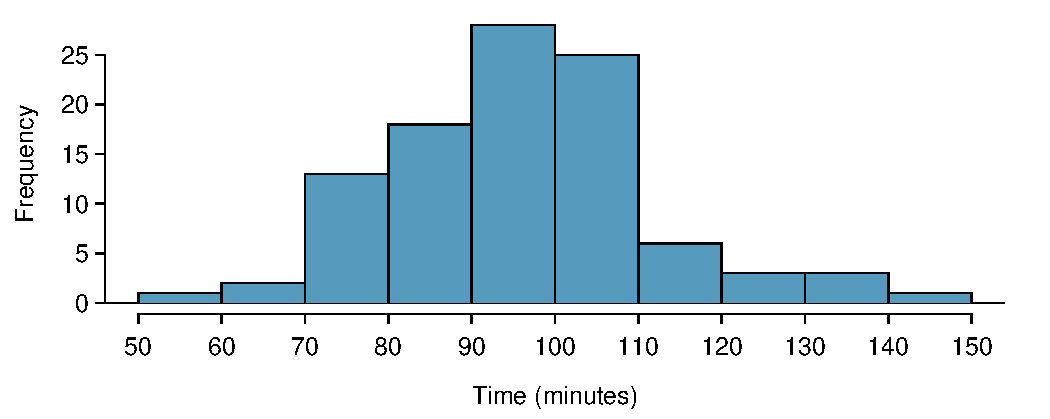
\includegraphics[width=\textwidth]{ch_distributions/figures/run10SampHistograms/run10SampHistograms} 
\caption{Histogram of \var{time} for a single sample of size 100. The average of the sample is in the mid-90s and the standard deviation of the sample $s\approx 16$ minutes.
\index{skew!example: moderate}}
\label{run10SampHistograms}
\end{figure}

From the random sample represented in \data{run10Samp}, we guessed the average time it takes to run 10 miles is 95.61 minutes. Suppose we take another random sample of 100 individuals and take its mean: 95.30 minutes. Suppose we took another (93.43 minutes) and another (94.16 minutes), and so on. If we do this many many times -- which we can do only because we have the entire population data set -- we can build up a \term{sampling distribution} for the sample mean when the sample size is 100, shown in Figure~\ref{netTime1000SamplingDistribution}.

\begin{figure}
   \centering
   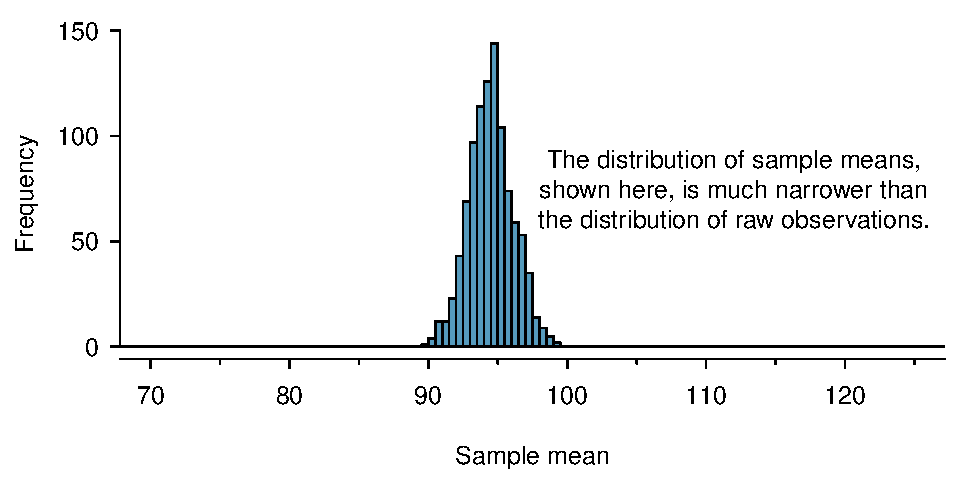
\includegraphics[width=0.93\textwidth]{ch_distributions/figures/netTime1000SamplingDistribution/netTime1000SamplingDistribution}
   \caption{A histogram of 1000 sample means for run time, where the samples are of size $n=100$. This histogram approximates the true sampling distribution of the sample mean, with mean $\mu_{\bar{x}}$ and standard deviation $\sigma_{\bar{x}}$.}
   \label{netTime1000SamplingDistribution}
\end{figure}

\begin{onebox}{Sampling distribution}
The sampling distribution represents the distribution of the point estimates based on samples of a fixed size from a certain population. It is useful to think of a point estimate as being drawn from such a distribution. Understanding the concept of a sampling distribution is central to understanding statistical inference.\end{onebox}

\textA{\pagebreak}

The sampling distribution shown in Figure~\ref{netTime1000SamplingDistribution} is unimodal and approximately symmetric. It is also centered exactly at the true population mean: $\mu=94.52$. Intuitively, this makes sense. The sample mean should be an unbiased estimator of the population mean. Because we are considering the distribution of the sample mean, we will use $\mu_{\bar{x}} = 94.52$ to describe the true mean of this distribution.

We can see that the sample mean has some variability around the population mean, which can be quantified using the standard deviation of this distribution of sample means. The standard deviation of the sample mean tells us how far the typical estimate is away from the actual population mean, 94.52 minutes. It also describes the typical \term{error} of a single estimate, and is denoted by the symbol $\sigma_{\bar{x}}$. 

\begin{onebox}{Standard deviation of an estimate}
The standard deviation associated with an estimate describes the typical error or uncertainty associated with the estimate.\end{onebox}

\begin{examplewrap}
\begin{nexample}{Looking at Figures~\ref{run10SampHistograms} and \ref{netTime1000SamplingDistribution}, we see that the standard deviation of the sample mean with $n=100$ is much smaller than the standard deviation of a single sample. Interpret this statement and explain why it is true.}The variation from one sample mean to another sample mean is much smaller than the variation from one individual to another individual. This makes sense because when we average over 100 values, the large and small values tend to cancel each other out. While many individuals have a time under 90 minutes, it would be unlikely for the \emph{average} of 100 runners to be less than 90 minutes.
\end{nexample}
\end{examplewrap}

\textA{\pagebreak}

\begin{exercisewrap}
\begin{nexercise}
(a) Would you rather use a small sample or a large sample when estimating a parameter? Why? (b) Using your reasoning from (a), would you expect a point estimate based on a small sample to have smaller or larger standard deviation than a point estimate based on a larger sample?\footnotemark
\end{nexercise}
\end{exercisewrap}
\footnotetext{(a) Consider two random samples: one of size 10 and one of size 1000. Individual observations in the small sample are highly influential on the estimate while in larger samples these individual observations would more often average each other out. The larger sample would tend to provide a more accurate estimate. (b) If we think an estimate is better, we probably mean it typically has less error. Based on (a), our intuition suggests that a larger sample size corresponds to a smaller standard deviation.}

When considering how to calculate the standard deviation of a sample mean, there is one problem: there is no obvious way to estimate this from a single sample. However, statistical theory provides a helpful tool to address this issue.

In the sample of 100 runners, the standard deviation of the sample mean is equal to one-tenth of the population standard deviation: $15.93/10 = 1.59$. In other words, the standard deviation of the sample mean based on 100 observations is equal to
\begin{eqnarray*}
SD_{\bar{x}} = \sigma_{\bar{x}} = \frac{\sigma_{x}}{\sqrt{n}} = \frac{15.93}{\sqrt{100}} = 1.59
\end{eqnarray*}
where $\sigma_{x}$ is the standard deviation of the individual observations. This is no coincidence. We can show mathematically that this equation is correct when the observations are independent  using the probability tools of Section~\ref{randomVariablesSection}.

\begin{onebox}{Computing SD for the sample mean}
Given $n$ independent observations from a population with standard deviation $\sigma$, the standard deviation of the sample mean is equal to \vspace{-1mm}
\begin{eqnarray}
SD_{\bar{x}} = \sigma_{\bar{x}} =  \frac{\sigma}{\sqrt{n}}
\label{seOfXBar}
\end{eqnarray}\vspace{-3mm}

A reliable method to ensure sample observations are independent is to conduct a simple random sample consisting of less than 10\% of the population.\index{standard error!single mean}\end{onebox}

\begin{exercisewrap}
\begin{nexercise}
The average of the runners' ages is 35.05 years with a standard deviation of $\sigma = 8.97$. A simple random sample of 100 runners is taken. (a)~What is the standard deviation of the sample mean? (b)~Would you be surprised to get a sample of size 100 with an average of 36~years?\footnotemark\end{nexercise}
\end{exercisewrap}
\footnotetext{(a) Use Equation~(\ref{seOfXBar}) with the population standard deviation to compute the standard deviation of the sample mean: $SD_{\bar{y}} = 8.97/\sqrt{100} = 0.90$ years. (b) It would not be surprising. 36 years is about 1 standard deviation from the true mean of 35.05. Based on the 68, 95 rule, we would get a sample mean at least this far away from the true mean approximately $100\% - 68\% = 32\%$ of the time.}

%library(openintro); library(xtable); data(run10); data(run10Samp); mean(run10Samp$age); sd(run10Samp$age); sd(run10$age, na.rm=TRUE)

\textA{\newpage}

\begin{exercisewrap}
\begin{nexercise}
(a) Would you be more trusting of a sample that has 100 observations or 400 observations? (b) We want to show mathematically that our estimate tends to be better when the sample size is larger. If the standard deviation of the individual observations is 10, what is our estimate of the standard deviation of the mean when the sample size is 100? What about when it is 400? (c) Explain how your answer to (b) mathematically justifies your intuition in part~(a).\footnotemark
\end{nexercise}
\end{exercisewrap}
\footnotetext{(a) Extra observations are usually helpful in understanding the population, so a point estimate with 400 observations seems more trustworthy. (b) The standard deviation of the mean when the sample size is 100 is given by $SD_{100} = 10/\sqrt{100} = 1$. For 400: $SD_{400} = 10/\sqrt{400} = 0.5$. The larger sample has a smaller standard deviation of the mean. (c) The standard deviation of the mean of the sample with 400 observations is lower than that of the sample with 100 observations. The standard deviation of $\bar{x}$ describes the typical error, and since it is lower for the larger sample, this mathematically shows the estimate from the larger sample tends to be better -- though it does not guarantee that every large sample will provide a better estimate than a particular small sample.}

%%
%%
\subsection{Examining the Central Limit Theorem}
\label{cltSection}

\index{Central Limit Theorem|(}

In Figure~\ref{netTime1000SamplingDistribution}, the sampling distribution of the sample mean looks approximately normally distributed. Will the sampling distribution of a mean always be nearly normal? To address this question, we will investigate three cases to see roughly when the approximation is reasonable.

We consider three data sets: one from a \emph{uniform} distribution, one from an \emph{exponential} distribution, and the other from a \emph{normal} distribution. These distributions are shown in the top panels of Figure~\ref{cltSimulations}. The uniform distribution is symmetric, and the exponential distribution may be considered as having moderate skew since its right tail is relatively short (few outliers).\index{skew!example: moderate}

\begin{figure}
   \centering
   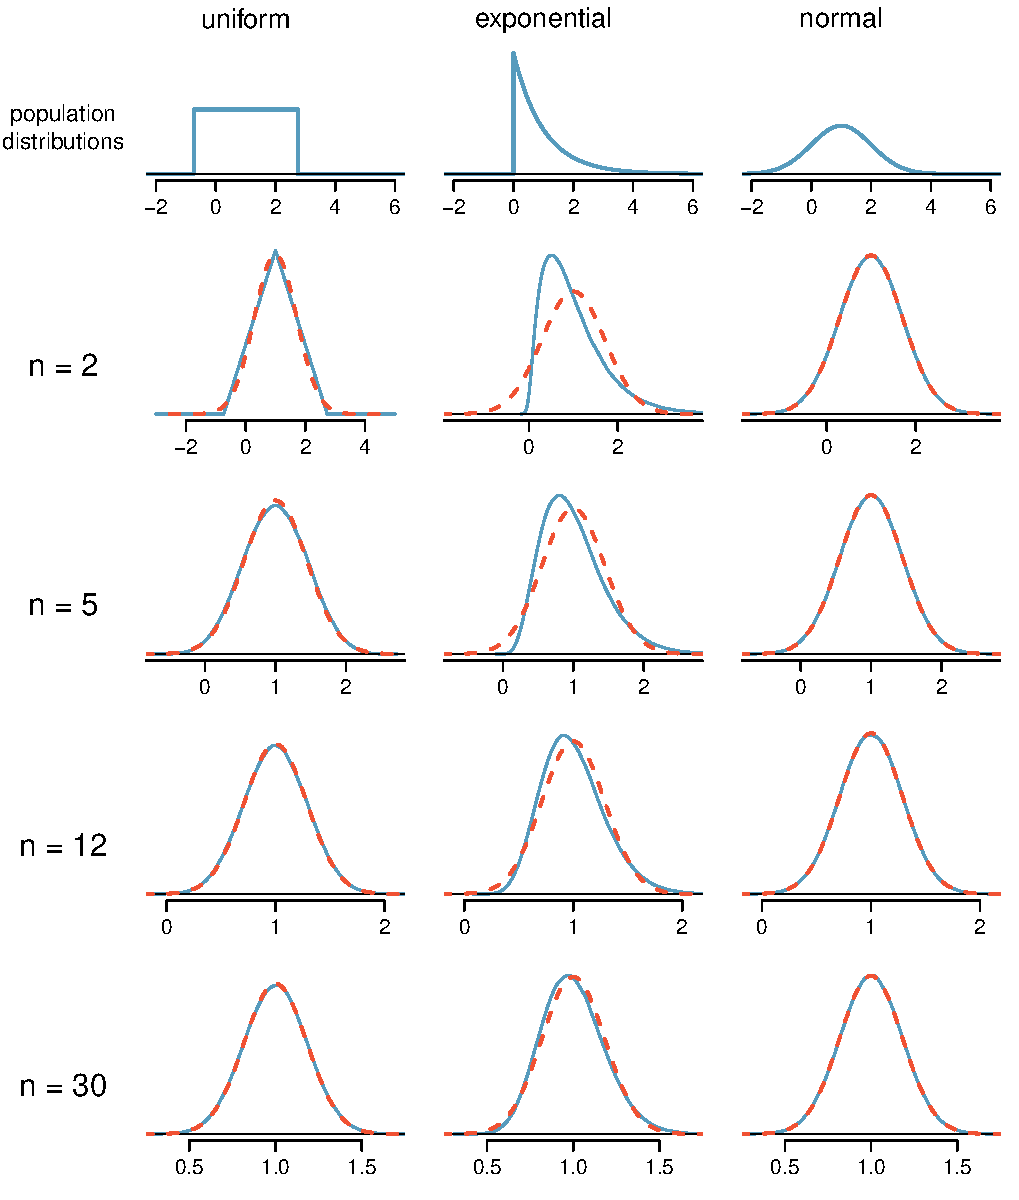
\includegraphics[width=\textwidth]{ch_distributions/figures/cltSimulations/cltSimulations}
   \caption{Sampling distributions for the mean at different sample sizes and for three different distributions. The dashed red lines show normal distributions.}
   \label{cltSimulations}
\end{figure}

The left panel in the $n=2$ row represents the sampling distribution of $\bar{x}$ if it is the sample mean of two observations from the uniform distribution shown. The dashed line represents the closest approximation of the normal distribution. Similarly, the center and right panels of the $n=2$ row represent the respective distributions of $\bar{x}$ for data from exponential and log-normal distributions.

\begin{exercisewrap}
\begin{nexercise}
Examine the distributions in each row of Figure~\ref{cltSimulations}. What do you notice about the sampling distribution of the mean as the sample size, $n$, becomes larger?\footnotemark
\end{nexercise}
\end{exercisewrap}
\footnotetext{The normal approximation becomes better as larger samples are used. However, in the case when the population is normally distributed, the normal distribution of the sample mean is normal for all sample sizes.}

\begin{examplewrap}
\begin{nexample}{In general, would normal approximation for a sample mean be appropriate when the sample size is at least 30?}
Yes, the sampling distributions when $n = 30$ all look very much like the normal distribution.

However, the more non-normal a population distribution, the larger a sample size is necessary for the sampling distribution to look nearly normal.
\end{nexample}
\end{examplewrap}

\begin{onebox}{Determining if the sample mean is normally distributed}
If the population is normal, the sampling distribution of $\bar{x}$ will be normal for any sample size. \\[2mm]
The less normal the population, the larger $n$ needs to be for the sampling distribution of $\bar{x}$ to be nearly normal. However, a good rule of thumb is that for almost all populations, the sampling distribution of $\bar{x}$ will be approximately normal if $n \ge 30$.\end{onebox}

This brings us to the \term{Central Limit Theorem}, the most fundamental theorem in Statistics.

\begin{onebox}{Central Limit Theorem}
When taking a random sample of independent observations from a population with a fixed mean and standard deviation, the distribution of $\bar{x}$ approaches the normal distribution as $n$ increases.\end{onebox}

\begin{examplewrap}
\begin{nexample}{Sometimes we do not know what the population distribution looks like. We have to infer it based on the distribution of a single sample. Figure~\ref{pokerProfitsCanApplyNormalToSampMean} shows a histogram of 20 observations. These represent winnings and losses from 20 consecutive days of a professional poker player. Based on this sample data, can the normal approximation be applied to the distribution of the sample mean?}
We should consider each of the required conditions.
\begin{itemize}
\setlength{\itemsep}{0mm}
\item[(1)] These are referred to as \term{time series data}, because the data arrived in a particular sequence. If the player wins on one day, it may influence how she plays the next. To make the assumption of independence we should perform careful checks on such data.
\item[(2)] The sample size is 20, which is smaller than 30.
\item[(3)] There are two outliers in the data, both quite extreme, which suggests the population may not be normal and instead may be very strongly skewed or have distant outliers. Outliers can play an important role and affect the distribution of the sample mean and the estimate of the standard deviation of the sample mean.
\end{itemize}
Since we should be skeptical of the independence of observations and the extreme upper outliers pose a challenge, we should not use the normal model for the sample mean of these 20 observations. If we can obtain a much larger sample, then the concerns about skew and outliers would no longer apply.
\end{nexample}
\end{examplewrap}

\begin{figure}[ht]
   \centering
   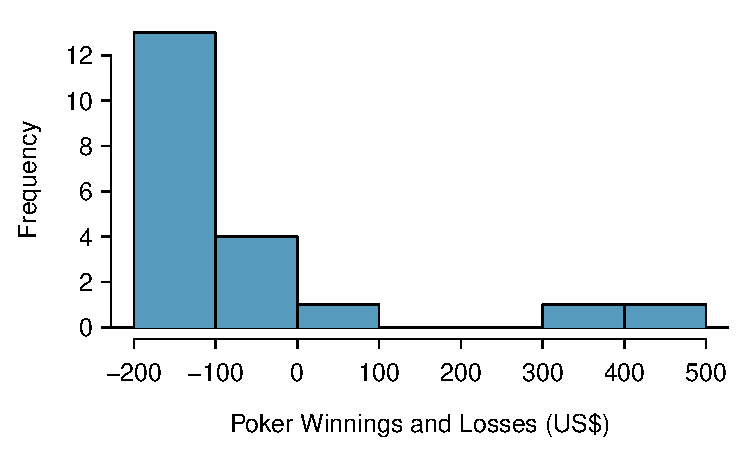
\includegraphics[height=58mm]{ch_distributions/figures/pokerProfitsCanApplyNormalToSampMean/pokerProfitsCanApplyNormalToSampMean}
   \caption{Sample distribution of poker winnings. These data include two very clear outliers. These are problematic when considering the normality of the sample mean. For example, outliers are often an indicator of very strong skew\index{skew!example: very strong}.}
   \label{pokerProfitsCanApplyNormalToSampMean}
\end{figure}

\begin{onebox}{Examine data structure when considering independence}
{Some data sets are collected in such a way that they have a natural underlying structure between observations, e.g. when observations occur consecutively. Be especially cautious about independence assumptions regarding such data sets.}
\end{onebox}

\begin{onebox}{Watch out for strong skew and outliers}
{Strong skew in the population is often identified by the presence of clear outliers in the data. If a data set has prominent outliers, then a larger sample size will be needed for the sampling distribution of $\bar{x}$ to be normal. There are no simple guidelines for what sample size is big enough for each situation. However, we can use the rule of thumb that, in general, an $n$ of at least 30 is sufficient for most cases.}
\index{skew!strongly skewed guideline}
\end{onebox}
\index{Central Limit Theorem|)}



%%
%%
\subsection{Normal approximation for the sampling distribution of $\bar{x}$}

At the beginning of this chapter, we used normal approximation for populations or for data that had an approximately normal distribution. When appropriate conditions are met, we can also use the normal approximation to estimate probabilities about a sample average. We must remember to verify that the conditions are met and use the mean $\mu_{\bar{x}}$ and standard deviation $\sigma_{\bar{x}}$ for the sampling distribution of the sample average.

\begin{onebox}{Three important facts about the distribution of a sample mean $\bar{x}$}
Consider taking a simple random sample from a large population.
\begin{enumerate}
\setlength{\itemsep}{0mm}
\item The mean of a sample mean is denoted by $\mu_{\bar{x}}$, and it is equal to $\mu$.
\item The SD of a sample mean is denoted by $\sigma_{\bar{x}}$, and it is equal to $\frac{\sigma}{\sqrt{n}}$.
\item When the population is normal or when $n\ge 30$, the sample mean closely follows a normal distribution. 
\end{enumerate}\end{onebox}

\textA{\pagebreak}

\begin{examplewrap}
\begin{nexample}{
In the 2012 Cherry Blossom 10 mile run, the average time for all of the runners is 94.52 minutes with a standard deviation of 8.97 minutes. The distribution of run times is approximately normal. Find the probabiliy that a randomly selected runner completes the run in less than 90 minutes.}Because the distribution of run times is approximately normal, we can use normal approximation.
\begin{align*}
&Z = \frac{x - \mu}{\sigma}=\frac{90-94.52}{8.97}=-0.504 \\
&P(Z < -0.504) = 0.3072
\end{align*}
There is a 30.72\% probability that a randomly selected runner will complete the run in less than 90~minutes.
\end{nexample}
\end{examplewrap}

\begin{examplewrap}
\begin{nexample}{
Find the probabiliy that the average of 20 runners is less than 90~minutes.}
Here, $n=20<30$, but the distribution of the population, that~is, the distribution of run times is stated to be approximately normal. Because of this, the sampling distribution will be normal for any sample size.
\begin{align*}
&\sigma_{\bar{x}}=\frac{\sigma}{\sqrt{n}}=\frac{8.97}{\sqrt{20}}=2.01 \\
&Z = \frac{\bar{x} - \mu_{\bar{x}}}{\sigma_{\bar{x}}}=\frac{90-94.52}{2.01}=-2.25\\
&P(Z < -2.25) = 0.0123
\end{align*}
There is a 1.23\% probability that the average run time of 20 randomly selected runners will be less than 90~minutes.
\end{nexample}
\end{examplewrap}

\begin{examplewrap}
\begin{nexample}{
The average of all the runners' ages is 35.05 years with a standard deviation of $\sigma = 8.97$. The distribution of age is somewhat skewed. What is the probability that a randomly selected runner is older than 37 years?}Because the distribution of age is skewed and is not normal, we cannot use normal approximation for this problem. In order to answer this question, we would need to look at all of the data.
\end{nexample}
\end{examplewrap}

\begin{exercisewrap}
\begin{nexercise}
What is the probability that the average of 50 randomly selected runners is greater than 37 years?\footnotemark
\end{nexercise}
\end{exercisewrap}
\footnotetext{Because $n=50\ge 30$, the sampling distribution of the mean is approximately normal, so we can use normal approximation for this problem. The mean is given as 35.05 years.
\begin{align*}
&\sigma_{\bar{x}}
	= \frac{\sigma}{\sqrt{n}}
	= \frac{8.97}{\sqrt{50}}=1.27
&&z=\frac{\bar{x}-\mu_{\bar{x}}}{\sigma_{\bar{x}}} = \frac{37-35.05}{1.27}=1.535
&&P(Z > 1.535) = 0.062
\end{align*}
There is a 6.2\% chance that the average age of 50 runners will be greater than 37.} 

\begin{onebox}{Remember to divide by $\sqrt{n}$}
When finding the probability that an \emph{average} or mean is greater or less than a particular value, remember to divide the standard deviation of the population by $\sqrt{n}$ to calculate the correct~SD.\end{onebox}

%%
%%
\subsection*{Section summary}

\begin{itemize}
\item The symbol $\bar{x}$ denotes the sample average.  $\bar{x}$ for any particular sample is a number.  However, $\bar{x}$ can vary from sample to sample.  The distribution of all possible values of $\bar{x}$ for repeated samples of a fixed size from a certain population is called the \term{sampling distribution} of $\bar{x}$.

\item The standard deviation of $\bar{x}$ describes the typical error or distance of the sample mean from the population mean.  It also tells us how much the sample mean is likely to vary from one random sample to another.  

\item The standard deviation of $\bar{x}$ will be \textit{smaller} than the standard deviation of the population by a factor of $\sqrt{n}$.  The larger the sample, the better the estimate tends to be.

\item Consider taking a simple random sample from a population with a fixed mean and standard deviation.  The \term{Central Limit Theorem} ensures that regardless of the shape of the original population, as the sample size increases, the distribution of the sample average $\bar{x}$ becomes more normal.  

\item Three important facts about the sampling distribution of the sample average $\bar{x}$:
\begin{itemize}\vspace{-1mm}
\setlength{\itemsep}{0mm}
\item The mean of a sample mean is denoted by $\mu_{\bar{x}}$, and it is equal to $\mu$. (\textit{center})
\item The SD of a sample mean is denoted by $\sigma_{\bar{x}}$, and it is equal to $\frac{\sigma}{\sqrt{n}}$.  (\textit{spread})
\item When the population is normal or when $n\ge 30$, the sample mean closely follows a normal distribution.   (\textit{shape})
\end{itemize}

\item These facts are used when solving the following two types of \textbf{normal approximation} problems involving a \emph{sample mean} or a \emph{sample sum}.  
\begin{itemize}
\item[A:] \textit{Find the probability that a sample average will be greater/less than a certain value}.
\begin{enumerate}\vspace{-1mm}
\setlength{\itemsep}{0mm}
\item Verify that the population is approximately normal or that $n \ge 30$.
\item Calculate the Z-score.  Use $\mu_{\bar{x}}=\mu$ and $\sigma_{\bar{x}}=\frac{\sigma}{\sqrt{n}}$ to standardize the sample average.  
\item Find the appropriate area under the normal curve.  
\end{enumerate}

\item[B:] \textit{Find the probability that a sample sum/total will be greater/less than a certain value}.
\begin{enumerate}\vspace{-1mm}
\setlength{\itemsep}{0mm}
\item Convert the sample sum into a sample average, using $\bar{x} = \frac{sum}{n}$.  
\item Do steps 1-3 from Part A above. 
\end{enumerate}
\end{itemize}
\end{itemize}



%__________________________________________
\section{Geometric distribution}
\label{geomDist}

\sectionintro{How long should we expect to flip a coin until it turns up \resp{heads}? Or how many times should we expect to roll a die until we get a \resp{1}? These questions can be answered using the geometric distribution. We first formalize each trial -- such as a single coin flip or die toss -- using the Bernoulli distribution, and then we combine these with our tools from probability (Chapter~\ref{probability}) to construct the geometric distribution.

%%
\subsection{Learning objectives}

\begin{enumerate}

\item Determine if a scenario is geometric.

\item Calculate the probabilities of the possible values of a geometric random variable.

\item Find and interpret the mean (expected value) of a geometric distribution.

\item Understand the shape of the geometric distribution.

\end{enumerate}
}

%%
\subsection{Bernoulli distribution}
\label{bernoulli}

\index{distribution!Bernoulli|(}

Stanley Milgram\index{Milgram, Stanley} began a series of experiments in 1963 to estimate what proportion of people would willingly obey an authority and give severe shocks to a stranger. Milgram found that about 65\% of people would obey the authority and give such shocks. Over the years, additional research suggested this number is approximately consistent across communities and time.\footnote{Find further information on Milgram's experiment at \par \ \ \hspace{0.2mm}\ \oiRedirect{textbook-milgram}{www.cnr.berkeley.edu/ucce50/ag-labor/7article/article35.htm}.}

Each person in Milgram's experiment can be thought of as a \term{trial}. We label a person a \term{success} if she refuses to administer the worst shock. A person is labeled a \term{failure} if she administers the worst shock. Because only 35\% of individuals refused to administer the most severe shock, we denote the \term{probability of a success} with $p=0.35$. The probability of a failure is sometimes denoted with $q=1-p$.

Thus, \resp{success} or \resp{failure} is recorded for each person in the study. When an individual trial only has two possible outcomes, it is called a \termsub{Bernoulli random variable}{distribution!Bernoulli}.

\begin{onebox}{Bernoulli random variable, descriptive}
A Bernoulli random variable has exactly two possible outcomes. We typically label one of these outcomes a ``success'' and the other outcome a ``failure''. We may also denote a success by \resp{1} and a failure by \resp{0}.\end{onebox}

\begin{onebox}{``success'' need not be something positive}
We chose to label a person who refuses to administer the worst shock a ``success'' and all others as ``failures''. However, we could just as easily have reversed these labels. The mathematical framework we will build does not depend on which outcome is labeled a success and which a failure, as long as we are consistent.\end{onebox}

Bernoulli random variables are often denoted as \resp{1} for a success and \resp{0} for a failure. In addition to being convenient in entering data, it is also mathematically handy. Suppose we observe ten trials:
\begin{center}
\resp{0} \resp{1} \resp{1} \resp{1} \resp{1} \resp{0} \resp{1} \resp{1} \resp{0} \resp{0}
\end{center}
Then the \term{sample proportion}, $\hat{p}$, is the sample mean of these observations:
\begin{eqnarray*}
\hat{p} = \frac{\text{\# of successes}}{\text{\# of trials}} = \frac{0+1+1+1+1+0+1+1+0+0}{10} = 0.6
\end{eqnarray*}
This mathematical inquiry of Bernoulli random variables can be extended even further. Because \resp{0} and \resp{1} are numerical outcomes, we can define the {mean} and {standard deviation} of a Bernoulli random variable.\footnote{If ${p}$ is the true probability of a success, then the mean of a Bernoulli random variable $X$ is given by
\begin{align*}
\mu = E[X] &= P(X=0)\times0 + P(X=1)\times1 \\
	&= (1-p)\times0 + p\times 1 = 0+p = p
\end{align*}
Similarly, the variance of $X$ can be computed:
\begin{align*}
\sigma^2 &= {P(X=0)(0-p)^2 + P(X=1)(1-p)^2} \\
	&= {(1-p)p^2 + p(1-p)^2} = {p(1-p)}
\end{align*}
The standard deviation is $\sigma=\sqrt{p(1-p)}$.}

\begin{onebox}{Bernoulli random variable, mathematical}
If $X$ is a random variable that takes value 1 with probability of success $p$ and 0 with probability $1-p$, then $X$ is a Bernoulli random variable with mean and standard deviation
\begin{align*}
\mu &= p
	&\sigma&= \sqrt{p(1-p)}
\end{align*}\end{onebox}

In general, it is useful to think about a Bernoulli random variable as a random process with only two outcomes: a success or failure. Then we build our mathematical framework using the numerical labels \resp{1} and \resp{0} for successes and failures, respectively.

\index{distribution!Bernoulli|)}


%%
\subsection{Geometric distribution}

\index{distribution!geometric|(}

\begin{examplewrap}
\begin{nexample}{Dr. Smith wants to repeat Milgram's experiments but she only wants to sample people until she finds someone who will not inflict the worst shock.\footnotemark\, If the probability a person will \emph{not} give the most severe shock is still 0.35 and the subjects are independent, what are the chances that she will stop the study after the first person? The second person? The third? What about if it takes her $n-1$ individuals who will administer the worst shock before finding her first success, i.e. the first success is on the $n^{th}$ person? (If the first success is the fifth person, then we say $n=5$.)} \label{waitForShocker}
The probability of stopping after the first person is just the chance the first person will not administer the worst shock: $1-0.65=0.35$. The probability it will be the second person is
\begin{eqnarray*}
&&P(\text{second person is the first to not administer the worst shock}) \\
&&\quad = P(\text{the first will, the second won't}) = (0.65)(0.35) = 0.228
\end{eqnarray*}
Likewise, the probability it will be the third person is $(0.65)(0.65)(0.35) = 0.148$.

If the first success is on the $n^{th}$ person, then there are $n-1$ failures and finally 1 success, which corresponds to the probability $(0.65)^{n-1}(0.35)$. This is the same as $(1-0.35)^{n-1}(0.35)$.
\end{nexample}
\end{examplewrap}
\footnotetext{This is hypothetical since, in reality, this sort of study probably would not be permitted any longer under current ethical standards.}

Example~\ref{waitForShocker} illustrates what is called the geometric distribution, which describes the waiting time until a success for \term{independent and identically distributed (iid)} Bernoulli random variables. In this case, the \emph{independence} aspect just means the individuals in the example don't affect each other, and \emph{identical} means they each have the same probability of success.

The geometric distribution from Example~\ref{waitForShocker} is shown in Figure~\ref{geometricDist35}. In general, the probabilities for a geometric distribution decrease \term{exponentially} fast.

\begin{figure}
\centering
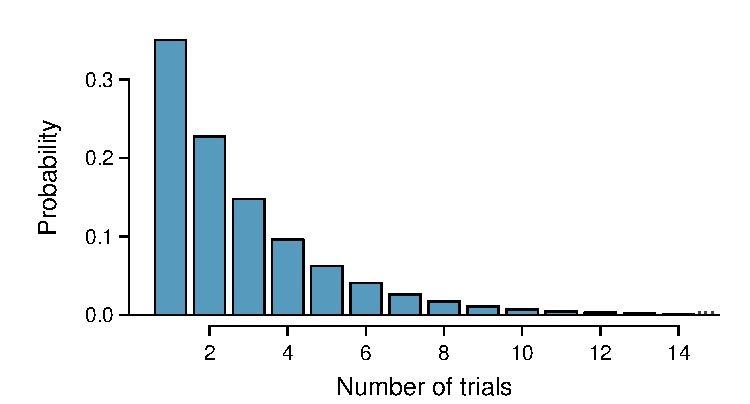
\includegraphics[width=0.77\textwidth]{ch_distributions/figures/geometricDist35/geometricDist35}
\caption{The geometric distribution when the probability of success is $p=0.35$.}
\label{geometricDist35}
\end{figure}

While this text will not derive the formulas for the mean (expected) number of trials needed to find the first success or the standard deviation or variance of this distribution, we present general formulas for each.

\begin{onebox}{Geometric distribution}
\index{distribution!geometric|textbf}
If the probability of a success in one trial is $p$ and the probability of a failure is $1-p$, then the probability of finding the first success in the $n^{th}$ trial is given by\vspace{-1.5mm}
\begin{eqnarray}
(1-p)^{n-1}p
\end{eqnarray}
The mean (i.e. expected value) and standard deviation of this wait time are \mbox{given by}\vspace{-2.5mm}
\begin{align}
\mu &= \frac{1}{p}
	&\sigma &= \sqrt{\frac{1-p}{p^2}}
\label{geomFormulas}
\end{align}\end{onebox}

It is no accident that we use the symbol $\mu$ for both the mean and expected value. The mean and the expected value are one and the same.

The left side of Equation~(\ref{geomFormulas}) says that, on average, it takes $1/p$ trials to get a success. This mathematical result is consistent with what we would expect intuitively. If the probability of a success is high (e.g. 0.8), then we don't usually wait very long for a success: $1/0.8 = 1.25$ trials on average. If the probability of a success is low (e.g. 0.1), then we would expect to view many trials before we see a success: $1/0.1 = 10$ trials.

\begin{exercisewrap}
\begin{nexercise}
The probability that an individual would refuse to administer the worst shock is said to be about 0.35. If we were to examine individuals until we found one that did not administer the shock, how many people should we expect to check? The first expression in Equation~(\ref{geomFormulas}) may be useful.\footnotemark
\end{nexercise}
\end{exercisewrap}
\footnotetext{We would expect to see about $1/0.35 = 2.86$ individuals to find the first success.}


\begin{examplewrap}
\begin{nexample}{What is the chance that Dr. Smith will find the first success within the first 4 people?} \label{marglimFirstSuccessIn4}
This is the chance it is the first ($n=1$), second ($n=2$), third ($n=3$), or fourth ($n=4$) person as the first success, which are four disjoint outcomes. Because the individuals in the sample are randomly sampled from a large population, they are independent. We compute the probability of each case and add the separate results:
\begin{eqnarray*}
&&P(n=1, 2, 3,\text{or}4) \\
	&& \quad = P(n=1)+P(n=2)+P(n=3)+P(n=4) \\
	&& \quad = (0.65)^{1-1}(0.35) + (0.65)^{2-1}(0.35) + (0.65)^{3-1}(0.35) + (0.65)^{4-1}(0.35) \\
	&& \quad = 0.82
\end{eqnarray*}
There is an 82\% chance that she will end the study within 4~people.
\end{nexample}
\end{examplewrap}

\begin{exercisewrap}
\begin{nexercise}
Determine a more clever way to solve Example~\ref{marglimFirstSuccessIn4}. Show that you get the same result.\footnotemark
\end{nexercise}
\end{exercisewrap}
\footnotetext{First find the probability of the complement: $P($no success in first 4~trials$) = 0.65^4 = 0.18$. Next, compute one minus this probability: $1-P($no success in 4 trials$) = 1-0.18 = 0.82$.}

\begin{examplewrap}
\begin{nexample}{Suppose in one region it was found that the proportion of people who would administer the worst shock was ``only'' 55\%. If people were randomly selected from this region, what is the expected number of people who must be checked before one was found that would be deemed a success? What is the standard deviation of this waiting time?} \label{onlyShocking55PercOfTheTimeExample}
A success is when someone will \textbf{not} inflict the worst shock, which has probability $p=1-0.55=0.45$ for this region. The expected number of people to be checked is $1/p = 1/0.45 = 2.22$ and the standard deviation is $\sqrt{(1-p)/p^2} = 1.65$.
\end{nexample}
\end{examplewrap}

\begin{exercisewrap}
\begin{nexercise}
Using the results from Example~\ref{onlyShocking55PercOfTheTimeExample}, $\mu = 2.22$ and $\sigma = 1.65$, would it be appropriate to use the normal model to find what proportion of experiments would end in 3 or fewer trials?\footnotemark
\end{nexercise}
\end{exercisewrap}
\footnotetext{No. The geometric distribution is always right skewed and can never be well-approximated by the normal model.}

The independence assumption is crucial to the geometric distribution's accurate description of a scenario. Mathematically, we can see that to construct the probability of the success on the $n^{th}$ trial, we had to use the Multiplication Rule for Independent Processes. It is no simple task to generalize the geometric model for dependent trials.

%%
\subsection*{Section summary}
Previously in this chapter we looked at the normal distribution as a model for \emph{numerical} data.  In the next sections of this chapter we turn our attention to \term{categorical variables} with two levels.

\begin{itemize}
\item It is useful to model yes/no, success/failure with the values 1 and 0, respectively.\footnote{Formally, we call such a variable a Bernoulli random variable.}  We call the \term{probability of success $p$ }and the \term{probability of failure $1-p$}.

\item When the trials are \term{independent} and the value of $p$ is constant, the probability of finding \term{the first success on the $n^{th}$ trial} is given by $(1-p)^{n-1}p$.  We can see the reasoning behind this formula as follows:  for the first success to happen on the $n^{th}$ trial, it has to \emph{not} happen the first $n-1$ trials (with probability $1-p$), and then happen on the $n^{th}$ trial (with probability $p$).  

\item When we consider the \emph{entire distribution} of possible values for the how long \emph{until} the first success, we get a discrete probability distribution known as the geometric distribution. The \term{geometric distribution} describes the waiting time \emph{until} the first success, when the trials are independent and the probability of success, $p$, is constant.

\item The geometric distribution is always \emph{right skewed} and, in fact, has no maximum value.  The probabilities, though, decrease exponentially fast.

\item Even though the geometric distribution has an infinite number of values, it has a well-defined \term{mean}, $\mu=\frac{1}{p}$.  If the probability of success is $\frac{1}{10}$, then \emph{on average}, it takes 10 trials until we see the first success.\footnote{The geometric distribution also has a well defined standard deviation given by $\sigma=\sqrt{\frac{(1-p)}{p^2}}$.}  

\item Note that when the trials are not independent, we can simply modify the geometric formula to find the probability that the first success happens on the $n^{th}$ trial. Instead of simply raising ($1-p$) to the $n-1$, multiply the appropriate \emph{conditional} probabilities.

\end{itemize}

%______________________________________________
\section[Binomial distribution]{Binomial distribution }
\label{binomialModel}

\index{distribution!binomial|(}

\sectionintro{
\noindent \learningobj{Learning objectives}
\begin{itemize}
\item Determine if a scenario is binomial. 

\item Calculate the probabilities of the possible values of a binomial random variable.

\item Calculate and interpret the mean (expected value) and standard deviation of the number of success in n binomial trials.

\item Determine whether a binomial distribution can be modeled as approximately normal.  If so, use normal approximation to estimate cumulative binomial probabilities.
\end{itemize}}

%%
\subsection{An example of a binomial distribution}

Take a second look at Guided Practice~\ref{noMoreThanOneFriendWSevereLungCondition} on page~\pageref{noMoreThanOneFriendWSevereLungCondition}. We asked many probability questions regarding this scenario that could be solved using the binomial formula. Instead of looking at it piecewise, we could describe the entire \emph{distribution} of possible values and their corresponding probabilities. Since there are 4 smoking friends, there are several possible outcomes for the number who might develop a severe lung condition in their lifetime: 0, 1, 2, 3, 4. We can make a distribution table as we did previously. Recall that the probability that a random smoker will develop a severe lung condition in her lifetime is about $0.3$.

\begin{table}[h]
\centering
\begin{tabular}{l l}
$x_i$ & $p_i$ \\
\hline
0 &  ${4\choose 0}(0.3)^0(0.7)^{4} = 0.240$ \vspace{1mm}\\
1 &  ${4\choose 1}(0.3)^1(0.7)^{3} = 0.412$  \vspace{1mm}\\
2 & ${4\choose 2}(0.3)^2(0.7)^{2} = 0.265$  \vspace{1mm}\\
3 & ${4\choose 3}(0.3)^3(0.7)^{1} = 0.076$  \vspace{1mm}\\
4 & ${4\choose 4}(0.3)^4(0.7)^{0} = 0.008$  \vspace{1mm}\\
\hline
\end{tabular}
\caption{Probability distribution for the number of 4 smoking friends who will develop a severe lung condition in their lifetime. This is a binomial distribution. Correcting for rounding error, the probabilities add up to~1, as they must for any probability distribution.}
\label{binomDistrSmokers}
\end{table}

\begin{figure}[h]
\centering
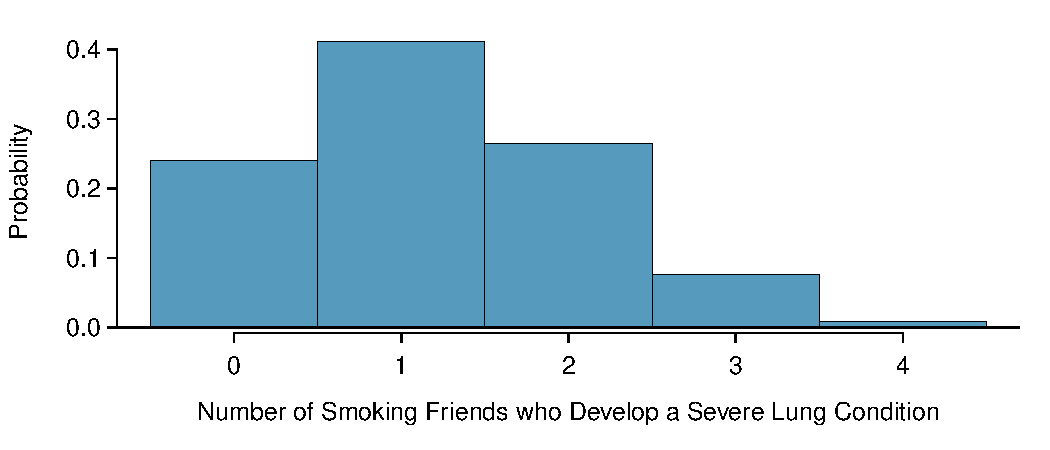
\includegraphics[width=0.9\textwidth]{ch_distributions/figures/smokingFriends4/smokingFriends4}
\caption{Distribution for the number of 4 smoking friends who will develop a severe lung condition.}
\label{smokingFriends4}
\end{figure}


\textA{\newpage}

%%
\subsection{The mean and standard deviation of a binomial distribution}

Since this is a probability distribution we could find the mean and standard deviation of it using the formulas from Chapter~\ref{probability}. Those formulas require a lot of calculations, so it is fortunate that there are shortcuts for the mean and the standard deviation of a binomial random variable.

\begin{onebox}{Mean and standard deviation of the binomial distribution}
For a binomial distribution with parameters $n$ and $p$, where $n$ is the number of trials and $p$ is the probability of a success, the mean and standard deviation of the number of observed successes are\vspace{-2mm}
\begin{align}
\mu_x &= np
	&\sigma_x &= \sqrt{np(1-p)}
\label{binomialStats}
\end{align}
\end{onebox}

\begin{examplewrap}
\begin{nexample}{If the probability that a random smoker will develop a severe lung condition in his or her lifetime is $0.3$ and you have 40 smoking friends, about how many would you expect to develop such a condition? What is the standard deviation of the number of people who would develop such a condition? Equation~(\ref{binomialStats}) may be useful.}
We are asked to determine the expected number (the mean) and the standard deviation, both of which can be directly computed from the formulas in Equation~(\ref{binomialStats}), as shown below. The exact distribution is shown in Figure~\ref{smokingFriends40}.
 \begin{align*}
\mu&=np = 40\times 0.3 = 12 \\
 \sigma &= \sqrt{np(1-p)} = \sqrt{40\times 0.3\times 0.7} = 2.9
\end{align*}
%Because very roughly 95\% of observations fall within 2 standard deviations of the mean, we would probably observe at least 6 but fewer than 18 of our smoking friends develop a severe lung condition in their lifetimes.
\end{nexample}
\end{examplewrap}

\begin{figure}[ht]
\centering
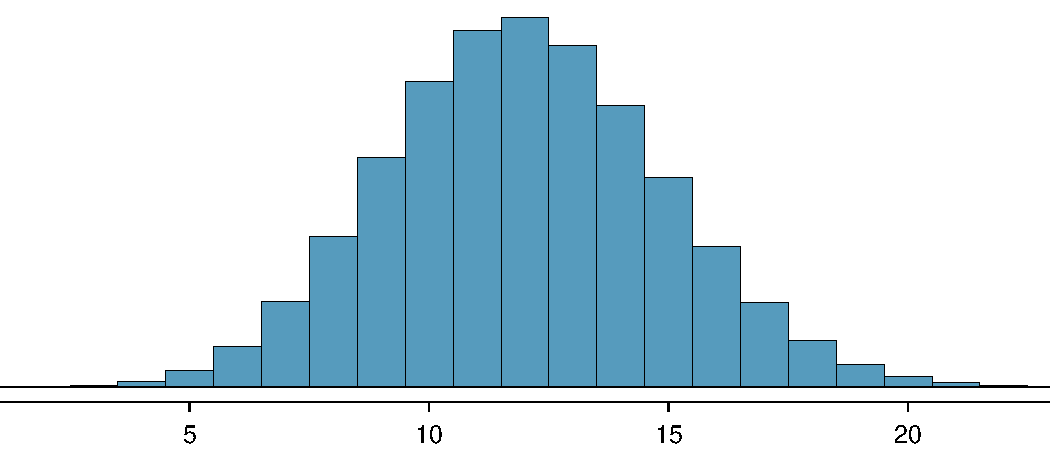
\includegraphics[width=0.9\textwidth]{ch_distributions/figures/smokingFriends40/smokingFriends40}
\caption{Distribution for the number of 40 smoking friends who will develop a severe lung condition, which looks very much like a normal distribution!} % A normal curve with mean 12 and standard deviation 2.9 has also been provided for a comparison.}
\label{smokingFriends40}
\end{figure}


%%
\subsection{Normal approximation to the binomial distribution}

\index{distribution!binomial!normal approximation|(}

The binomial formula is cumbersome when the sample size ($n$) is large, particularly when we consider a range of observations. Suppose we wanted to find the probability that at least 25 of 40 smoking friends will develop a severe lung condition. We would need to use the binomial formula with $k=25$, $k=26$, $k=27$, ..., $k=40$. That's a lot of work! In some cases we may use the normal distribution as an easier and faster way to estimate binomial probabilities. While a normal approximation for the distribution in Figure~\ref{smokingFriends4} would not be appropriate, it would not be too bad for the distribution in Figure~\ref{smokingFriends40}.

\begin{examplewrap}
\begin{nexample}{Approximately 20\% of the US population smokes cigarettes. A local government believed their community had a lower smoker rate and commissioned a survey of 400 randomly selected individuals. The survey found that only 60 of the 400 participants smoke cigarettes. If the true proportion of smokers in the community was really 20\%, what is the probability of observing 60 or fewer smokers in a sample of 400 people?}\label{exactBinomialForN400P20SmokerExample}
We leave the usual verification that the four conditions for the binomial model are valid as an exercise.

The question posed is equivalent to asking, what is the probability of observing $k=0$, 1, ..., 59, or 60 smokers in a sample of $n=400$ when $p=0.20$? We can compute these 61 different probabilities and add them together to find the answer:
\begin{align*}
&P(k=0\text{ or }k=1\text{ or } \cdots \text{ or } k=60) \\
	&\qquad= P(k=0) + P(k=1) + \cdots + P(k=60) \\
	&\qquad=0.0061
\end{align*}
If the true proportion of smokers in the community is $p=0.20$, then the probability of observing 60 or fewer smokers in a sample of $n=400$ is less than 0.0061.
\end{nexample}
\end{examplewrap}

The computations in Example~\ref{exactBinomialForN400P20SmokerExample} are tedious and long. In general, we should avoid such work if an alternative method exists that is faster, easier, and still accurate. Recall that calculating probabilities of a range of values is much easier in the normal model. We might wonder, is it reasonable to use the normal model in place of the binomial distribution? Surprisingly, yes, if certain conditions are met.

\begin{exercisewrap}
\begin{nexercise}
Here we consider the binomial model when the probability of a success is $p=0.10$. Figure~\ref{fourBinomialModelsShowingApproxToNormal} shows four hollow histograms for simulated samples from the binomial distribution using four different sample sizes: $n=10$, 30, 100, 300. What happens to the shape of the distributions as the sample size increases? What distribution does the last hollow histogram resemble?\footnotemark
\end{nexercise}
\end{exercisewrap}
\footnotetext{The distribution is transformed from a blocky and skewed distribution into one that rather resembles the normal distribution in last hollow histogram}

\begin{figure}[h]
\centering
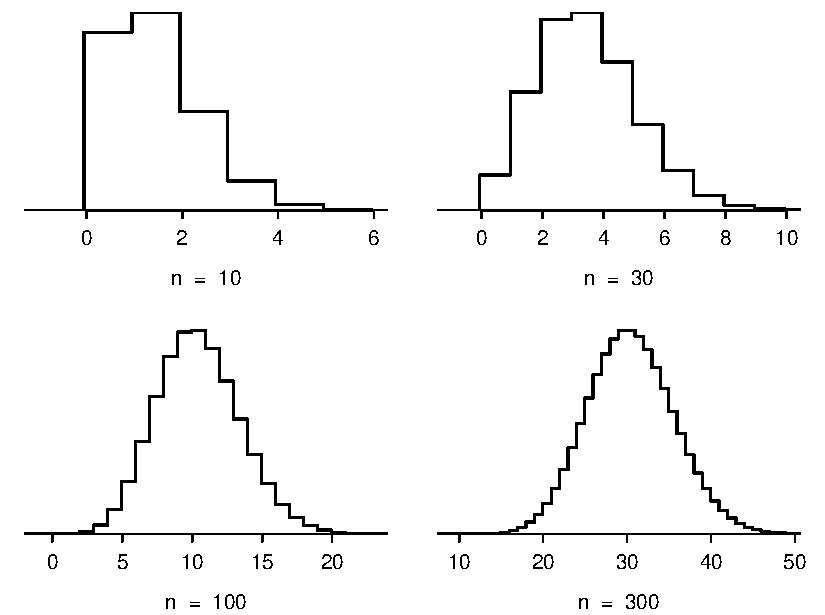
\includegraphics[width=0.95\textwidth]{ch_distributions/figures/fourBinomialModelsShowingApproxToNormal/fourBinomialModelsShowingApproxToNormal}
\caption{Hollow histograms of samples from the binomial model when $p=0.10$. The sample sizes for the four plots are $n=10$, 30, 100, and 300, respectively.}
\label{fourBinomialModelsShowingApproxToNormal}
\end{figure}

\begin{onebox}{Normal approximation of the binomial distribution}
The binomial distribution with probability of success $p$ is nearly normal when the sample size $n$ is sufficiently large that $np\ge 10$ and $n(1-p)\ge 10$. The approximate normal distribution has parameters corresponding to the mean and standard deviation of the binomial distribution:\vspace{-1.5mm}
\begin{align*}
\mu &= np
&&\sigma= \sqrt{np(1-p)}
\end{align*}\end{onebox}

The normal approximation may be used when computing the range of many possible successes. For instance, we may apply the normal distribution to the setting described in Example~\ref{exactBinomialForN400P20SmokerExample}.

\textA{\newpage}

\begin{examplewrap}
\begin{nexample}{Use the normal approximation to estimate the probability of observing 60 or fewer smokers in a sample of 400, if the true proportion of smokers is $p=0.20$.}\label{approxBinomialForN400P20SmokerExample}
As in Example~\ref{exactBinomialForN400P20SmokerExample},  we leave it to the reader to show that the binomial model is reasonable for this context. However, we will verify that both $np$ and $n(1-p)$ are at least 10 so we can apply the normal model:
\begin{align*}
np&=400(0.20)=80\ge 10
&
n(1-p)&=400(0.8)=320\ge 10
\end{align*}
With these conditions checked, we may use the normal approximation in place of the binomial distribution with the following mean and standard deviation:
\begin{align*}
\mu &= np = 400(0.2)=80
&
\sigma &= \sqrt{np(1-p)} = \sqrt{400(0.2)(0.8)}= 8
\end{align*}
We want to find the probability of observing 60 or fewer smokers using this model. We know that this probability will be small because 60 is more than 2 standard deviations below the mean:
\begin{center}
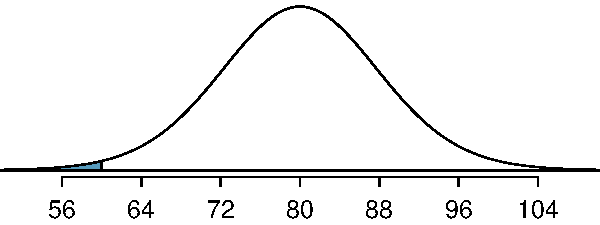
\includegraphics[width=0.5\textwidth]{ch_distributions/figures/smallTownSmokers/smallTownSmokers}
\end{center}
Next, we compute the Z-score as $Z=\frac{60 - 80}{8} = -2.5$ to find the shaded area in the picture: $P(Z < -2.5) = 0.0062$. This probability of 0.0062 using the normal approximation is remarkably close to the true probability of 0.0061 from the binomial distribution!
\end{nexample}
\end{examplewrap}

\begin{exercisewrap}
\begin{nexercise}
Use normal approximation, if applicable, to estimate the probability of getting greater than 15 sixes in 100 rolls of a fair die.\footnotemark
\end{nexercise}
\end{exercisewrap}
\footnote{$np=100\times 1/6=16.7\ge 10$ and 
$n(1-p)=100\times 5/6=83.3\ge 10$  

$\mu=np=100(1/6)=16.7; \sigma=\sqrt{np(1-p)}=\sqrt{100\times (1/6)(5/6)}=3.7$ 

$Z=\frac{15 - 16.7}{3.7} = -0.46$. 

$P(Z > -0.46) = 0.677$
}


%%
\subsection{The normal approximation breaks down on small intervals (special topic)}

\begin{onebox}{The normal approximation may fail on small intervals}
{The normal approximation to the binomial distribution tends to perform poorly when estimating the probability of a small range of counts, even when the conditions are met.}
\end{onebox}

Suppose we wanted to compute the probability of observing 69, 70, or 71 smokers in 400 when $p=0.20$. With such a large sample, we might be tempted to apply the normal approximation and use the range 69 to 71. However, we would find that the binomial solution and the normal approximation notably differ:
\begin{align*}
\text{Binomial:}&\ 0.0703
&\text{Normal:}&\ 0.0476
\end{align*}
We can identify the cause of this discrepancy using Figure~\ref{normApproxToBinomFail}, which shows the areas representing the binomial probability (outlined) and normal approximation (shaded). Notice that the width of the area under the normal distribution is 0.5 units too slim on both sides of the interval. The binomial distribution is a discrete distribution, and the each bar is centered over an integer value. Looking closely at Figure~\ref{normApproxToBinomFail}, we can see that the bar corresponding to 69 begins at 68.5 and ends at 69.5, the bar corresponding to 70 begins at 69.5 and ends at 70.5, etc.

\begin{figure}[h]
\centering
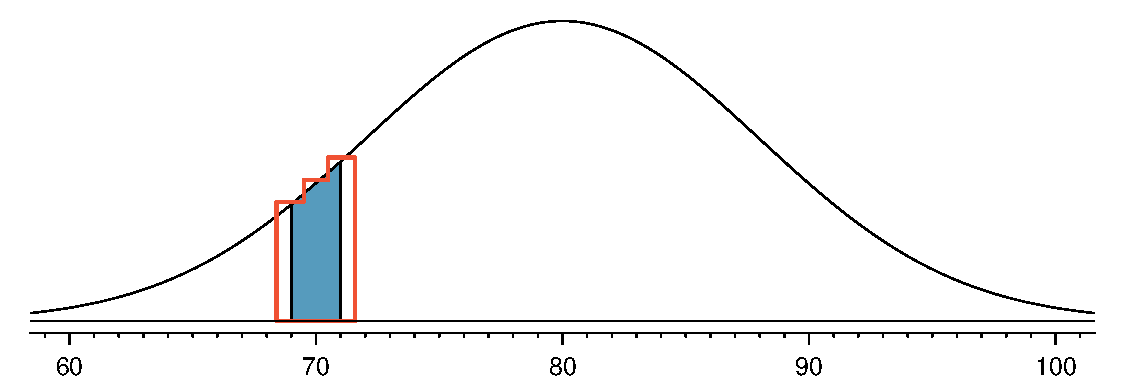
\includegraphics[width=\textwidth]{ch_distributions/figures/normApproxToBinomFail/normApproxToBinomFail}
\caption{A normal curve with the area between 69 and 71 shaded. The outlined area from 68.5 to 71.5 represents the exact binomial probability.}
\label{normApproxToBinomFail}
\end{figure}

\Comment{had to remove a the, from the accuracy to make fit on one line}

\begin{onebox}{Improving accuracy of the normal approximation to the binomial distribution}
The normal approximation to the binomial distribution for intervals of values is usually improved if cutoff values for the lower end of a shaded region are reduced by 0.5 and the cutoff value for the upper end are increased by 0.5. This correction is called the continuity correction and accounts for the fact that the binomial distribution is discrete.\end{onebox}

\begin{examplewrap}
\begin{nexample}{Use the method described to find a more accurate estimate for the probability of observing 69, 70, or 71 smokers in 400 randomly selected people when $p=0.20$.}
Instead of standardizing 69 and 71, we will standardize 68.5 and 71.5:
\begin{align*}
Z_{left} &= \frac{68.5-80}{8} = -1.4375 \\
Z_{right} &= \frac{71.5-80}{8} = -1.0625 \\
P(-1.4375 &< Z < -1.0625) = 0.0687
\end{align*}
The probability 0.0687 is much closer to the true value of 0.0703 than the previous estimate of 0.0476 we calculated using normal approximation without the continuity correction.
\end{nexample}
\end{examplewrap}

It is always possible to apply the continuity correction when finding a normal approximation to the binomial distribution. However, when $n$ is very large or when the interval is wide, the benefit of the modification is limited since the added area becomes negligible compared to the overall area being calculated.

\index{distribution!binomial!normal approximation|)}
\index{distribution!binomial|)}

%%
\subsection*{Section summary}

In the previous chapter, we introduced the binomial formula to find the probability of exactly $k$ successes in $n$ trials for an event that has probability $p$ of success.  Instead of looking at this scenario piecewise, we can describe the entire \textit{distribution} of the number of successes and their corresponding probabilities.  
\begin{itemize}
\item The distribution of the \textit{number of successes} in $n$ independent trials or in a random sample of size $n$ gives rise to a \term{binomial distribution}.  

\item To write out a binomial probability \textbf{distribution table}, list all possible values for $k$, the number of successes, then use the binomial formula to find the probability of each of those values.  

\item Because a binomial distribution can be thought of as the \emph{sum} of a bunch of 0s and 1s, the \term{Central Limit Theorem} applies.  As $n$ gets larger, the shape of the binomial distribution becomes more normal.  

\item  We call the rule of thumb for when the binomial distribution can be well modeled with a normal distribution the \term{success-failure} condition.  The success-failure condition is met when there are at least 10 successes and 10 failures, or when $np\ge 10$ and $n(1-p)\ge 10$.

\item If \textit{X} follows a binomial distribution with parameters $n$ and $p$, then:
\begin{itemize}\vspace{-1mm}
\setlength{\itemsep}{0mm}
\item The mean is given by $\mu_x = np$. \quad (\emph{center})
\item The standard deviation is given by $\sigma_x = \sqrt{np(1-p)}$. \quad (\emph{spread})
\item When $np\ge 10$ and $n(1-p)\ge 10$, the binomial distribution is approximately normal.  \quad (\emph{shape})
\end{itemize}

\item It is often easier to use \term{normal approximation to the binomial distribution} rather than evaluate the binomial formula many times. These three properties of the binomial distribution are used when solving the following type of problem.  
\\
\\ \textit{Find the probability of getting more than / fewer than X yeses in $n$ trials or in a sample of size $n$}.  
\begin{enumerate}\vspace{-1mm}
\setlength{\itemsep}{0mm}
\item Identify $n$ and $p$. Verify than $np\ge 10$ and $n(1-p)\ge 10$, which implies that normal approximation is reasonable. 
\item Calculate the Z-score.  Use $\mu_x = np$ and $\sigma_x = \sqrt{np(1-p)}$ to standardize the X value.  
\item Find the appropriate area under the normal curve.   
\end{enumerate}

\end{itemize}



%______________________________________________
\section[Sampling distribution of a sample proportion]{Sampling distribution of a sample proportion }
\label{distributionphat}

\sectionintro{
The binomial distribution shows us the distribution of number of successes in $n$ trials. Often, we are interested in the \emph{proportion} of successes rather than the number of successes. We would like to answer questions such as the following:

\begin{itemize}
\item Approximately 20\% of the US population smokes cigarettes. A random sample of size 400 from a particular county found that 15\% of the sample smoked. If the smoking rate in this county really is 20\%, what is the probability that the sample would contain 15\% or fewer smokers?  

\item Given a population that is 50\% male, what is the probability that a sample of size of 200 people would consist of more than 55\% males?

\end{itemize}

%%
\subsection*{Learning objectives}
\begin{enumerate}
\item Describe the center, spread, and shape of the sampling distribution of a sample proportion.


\item Recognize the relationship between the distribution of a sample proportion and the corresponding binomial distribution. 

\item Identify and explain the conditions for using normal approximation involving a sample proportion. Recognize that the Central Limit Theorem applies in the case of proportions/counts as well as means/sums.

\item Verify that the conditions for normal approximation are met and carry out normal approximation involving a sample proportion or sample count.

\end{enumerate}
}


%%
\subsection{The mean and standard deviation of $\hat{p}$}

To answer these questions, we investigate the distribution of the sample proportion $\hat{p}$. In the last section we saw that the \emph{number} of smokers in a sample of size 400 follows a binomial distribution with $p=0.2$ and $n=400$ that is centered on 80 and has standard deviation 8. What does the distribution of the \emph{proportion} of smokers in a sample of size 400 look like?  To convert from a count to a proportion, we divide the count (i.e.~number of~yeses) by the sample size, $n = 400$. For example, 60 becomes $60/400 = 0.15$ as a proportion and 61 becomes $61/400 = 0.1525$. 

We can find the general formula for the mean (expected value) and standard deviation of a sample proportion $\hat{p}$ using our tools that we've learned so far. To get the sample mean for $\hat{p}$, we divide the binomial mean $\mu_{binomial} = np$ by $n$:
\begin{align*}
\mu_{\hat{p}} = \frac{\mu_{binomial}}{n} = \frac{np}{n} = p
\end{align*}
As one might expect, the sample proportion $\hat{p}$ is centered on the true proportion $p$. Likewise, the standard deviation of $\hat{p}$ is equal to the standard deviation of the binomial distribution divided by $n$:
\begin{align*}
\sigma_{\hat{p}}
	= \frac{\sigma_{binomial}}{n}
	= \frac{\sqrt{np(1-p)}}{n}
	= \sqrt{\frac{p(1-p)}{n}}
\end{align*}

\begin{onebox}{Mean and standard deviation of a sample proportion}
The mean and standard deviation of the sample proportion describe the center and spread of the distribution of all possible sample proportions $\hat{p}$ from a random sample of size $n$ with true population proportion $p$.
\begin{align*}
\mu_{\hat{p}} &= p
	& \sigma_{\hat{p}}&= \sqrt{\frac{p(1-p)}{n}}
	\vspace{1mm}
\end{align*}\end{onebox}

%Because the distribution of $\hat{p}$ is centered at $p$, the sample proportion is said to be an \hiddenterm{unbiased estimator} of $p$.

In analyses, we think of the formula for the standard deviation of a sample proportion, $\sigma_{\hat{p}}$, as describing the uncertainty associated with the estimate $\hat{p}$. That is, $\sigma_{\hat{p}}$ can be thought of as a way to quantify the typical \hiddenterm{error} in our sample estimate $\hat{p}$ of the true proportion $p$. Understanding the variability of statistics such as $\hat{p}$ is a central component in the study of statistics.

%\begin{enumerate}
%\setlength{\itemsep}{0mm}
%\item The average spread of the distribution of all possible values of $\hat{p}$ 
%\item The average \emph{error} of the sample proportion $\hat{p}$, that~is, the average deviation between a particular sample $\hat{p}$ and the true population $p$. 
%\end{enumerate}

\begin{examplewrap}
\begin{nexample}{If the rate of smoking in the county is really 20\%, find and interpret the mean and standard deviation of the sample proportion for a sample of size 400.}
The mean of the sample proportion is the population proportion: 0.20. That is, if we took many, many samples and calculated $\hat{p}$, these values would average out to $p = 0.20$.

The standard deviation of $\hat{p}$ is described by the standard deviation for the proportion:
\begin{align*}
\sigma_{\hat{p}}
	= \sqrt{\frac{p(1-p)}{n}}
	= \sqrt{\frac{0.2 \times 0.8}{400}}
	= .02
\end{align*}
The sample proportion will typically be about 0.02 or 2\% away from the true proportion of $p = 0.20$. We'll become more rigorous about quantifying how close $\hat{p}$ will tend to be to $p$ in Chapter~\ref{foundationsForInference}.
\end{nexample}
\end{examplewrap}

%%
\subsection{The Central Limit Theorem revisited}

In section ~\ref{distributionofxbar}, we saw the Central Limit Theorem, which states that for large enough $n$, the sample mean $\bar{x}$ is normally distributed.

A natural question is, what does this have to do with sample proportions? In~fact, a~lot! A sample proportion can be written down as a sample mean. For example, suppose we have 3 successes in 10 trials. If we label each of the 3 success as a 1 and each of the 7 failures as a 0, then the sample proportion is the same as the sample mean:
\begin{align*}
\hat{p}
	= \frac{1 + 0 + 0 + 1 + 1 + 0 + 0 + 0 + 0 + 0}{10}
	= \frac{3}{10}
	= 0.3
\end{align*}
That is, the distribution of the sample proportion is governed by the Central Limit Theorem, and the Central Limit Theorem is what ties much of the statistical theory we will see together.


\begin{onebox}{Three important facts about the distribution of a sample proportion $\hat{p}$}
Consider taking a simple  random sample from a large population.
\begin{enumerate}
\setlength{\itemsep}{0mm}
\item The mean of a sample proportion is $p$.
\item The SD of a sample proportion is $\sqrt{\frac{p(1-p)}{n}}$.
\item When $np \geq 10$ and $n(1-p) \geq 10$, the sample proportion closely follows a normal distribution. 
\end{enumerate}\end{onebox}

Using these facts, we can now answer the two questions posed at the beginning of this section.


\textA{\pagebreak}

%%
\subsection{Normal approximation for the distribution of $\hat{p}$}

\begin{examplewrap}
\begin{nexample}{Find the probability that less than 15\% of the sample of 400 people will be smokers if the true proportion is 20\%.}
In the previous section we verified that $np$ and $n(1-p)$ are at least 10. The mean of the sample proportion is 0.20 and the standard deviation for the sample proportion is given by $\sqrt{\frac{0.2(1-0.2)}{400}}=0.02$. We can find a Z-score and use our calculator to find the probability:
\begin{align*}
Z &= \frac{\hat{p} - \mu_{\hat{p}}}{\sigma_{\hat{p}}} = \frac{0.15 - 0.20}{0.02} = -2.5 \\
P(&Z < 2.5) = 0.0062
\end{align*}
We leave it to the reader to construct a figure for this example.
\label{smokers}
\end{nexample}
\end{examplewrap}
\footnotetext{First, verify the conditions: $np = 200 \times 0.5 = 100 \ge 10$ and $n(1-p) = 200 \times 0.5 = 100 \ge 10$, so the normal approximation is reasonable. Next we find the mean and standard deviation of $\hat{p}$:
\begin{align*}
\mu_{\hat{p}} &= p = 0.50
	& \sigma_{\hat{p}} &= \sqrt{\frac{p(1-p)}{n}}
		= \sqrt{\frac{0.5 \times 0.5}{200}}
		= 0.0354
\end{align*}
Then we find a Z-score and find the upper tail of the normal distribution:
\begin{align*}
Z = \frac{\hat{p} - \mu_{\hat{p}}}{\sigma_{\hat{p}}} = \frac{0.55 - 0.5}{0.0354} = 1.412
\qquad \rightarrow \qquad
P(Z > 1.412) = 0.07
\end{align*}
The probability of getting a sample proportion of 55\% or greater is about 0.07.}


\begin{examplewrap}
\begin{nexample}{The probability 0.0062 is the same probability we calculated when we found the probability of getting 60 or fewer smokers out of 400! Why is this?}
Notice that $60/400=0.15$. Using the binomial distribution to find the probability of 60 or fewer smokers in the sample is equivalent to using the probability that $\hat{p}$ will be less than or equal to 15\%.
\end{nexample}
\end{examplewrap}

\begin{exercisewrap}
\begin{nexercise}Given a population that is 50\% male, what is the probability that a sample of size 200 would have greater than 55\% males?  Remember to verify that conditions for normal approximation are met.\footnotemark
\end{nexercise}
\end{exercisewrap}

%%
\subsection*{Section summary}

The binomial distribution shows the distribution of the number of successes in $n$ trials.  Often, we are interested in the \textit{proportion} of successes rather than the \textit{number} of successes.
\begin{itemize}
\item To convert from "number of yeses" to "proportion of yeses" we simply divide the number by $n$.  The sampling distribution of the sample proportion $\hat{p}$ is identical to the binomial distribution with a change of scale, i.e. different mean and different SD, but same shape.

\item The same \term{success-failure condition} for the binomial distribution holds for a sample proportion $\hat{p}$.

\item Three important facts about the sampling distribution of the sample proportion $\hat{p}$:
\begin{itemize}\vspace{-1mm}
\item The mean of a sample proportion is denoted by $\mu_{\hat{p}}$, and it is equal to $p$.  (\textit{center})
\item The SD of a sample proportion is denoted by $\sigma_{\hat{p}}$, and it is equal to $\sqrt{\frac{p(1-p)}{n}}$.  (\textit{spread})
\item When $np\ge 10$ and $n(1-p)\ge 10$, the distribution of the sample proportion will be approximately normal.   (\textit{shape})
\end{itemize}

\item We use these properties when solving the following type of \term{normal approximation} problem involving a sample proportion.  
\emph{Find the probability of getting more / less than $x$\% yeses in a sample of size $n$}.
\begin{enumerate}\vspace{-1mm}
\setlength{\itemsep}{0mm}
\item Identify $n$ and $p$. Verify than $np\ge 10$ and $n(1-p)\ge 10$, which implies that normal approximation is reasonable. 
\item Calculate the Z-score.  Use $\mu_{\hat{p}} = p$ and $\sigma_{\hat{p}} = \sqrt{\frac{p(1-p)}{n}}$ to standardize the sample proportion.  
\item Find the appropriate area under the normal curve.  \end{enumerate}

\end{itemize}


%______________________________________________
\section{Chapter Highlights}
\addcontentsline{toc}{section}{Chapter Highlights}
This chapter began by introducing the normal distribution.  A common thread that ran through this chapter is the use of the \term{normal approximation} in various contexts.  
The key steps are included for each of the normal approximation scenarios below.

\begin{enumerate}
\item Normal approximation for \term{data}:  
\\- Verify that population is approximately normal.
\\- Use the given mean $\mu$ and SD $\sigma$ to find the Z-score for the given $x$ value.
\item Normal approximation for a \term{sample mean/sum}:  
\\Verify that population is approximately normal or that $n\ge 30$.
\\Use $\mu_{\bar{x}}=\mu$ and $\sigma_{\bar{x}}=\frac{\sigma}{\sqrt{n}}$ to find the Z-score for the given/calculated sample mean.
\item Normal approximation for the \term{number of successes} (binomial):  
\\- Verify that $np\ge 10$ and $n(1-p)\ge 10$.
\\- Use $\mu_x = np$ and $\sigma_x = \sqrt{np(1-p)}$ to find the Z-score for the given number of successes.  
\item Normal approximation for a \term{sample proportion}:  
\\- Verify that $np\ge 10$ and $n(1-p)\ge 10$.
\\- Use $\mu_{\hat{p}} = p$ and $\sigma_{\hat{p}} = \sqrt{\frac{p(1-p)}{n}}$ to find the Z-score for the given sample proportion.
\item Normal approximation for the \term{sum of two independent random variables}:
\\- Verify that each random variable is approximately normal.
\\- Use $E(X+Y)=E(X)+E(Y)$ and $SD(X+Y)=\sqrt{(SD(X))^2+(SD(Y))^2}$ to find the Z-score for the given sum.
\end{enumerate}
Cases 1 and 2 apply to \term{numerical} variables, while cases 3 and 4 are for \term{categorical} yes/no variables.  Case 5 applies to both numerical and categorical variables.
\\
\\Note that in the binomial case and in the case of proportions, we never look to see if the \emph{population} is normal.  That would not make sense because the ``population" is simply a bunch of no/yes, 0/1 values and could not possibly be normal.
\\
\\The \term{Central Limit Theorem} is the mathematical rule that ensures that when the sample size is sufficiently large, the sample mean/sum and sample proportion/count will be approximately normal.  

